% REMEMBER: You must not plagiarise anything in your report. Be extremely careful.
\documentclass{l4proj}

    
%==============================================================================
% Put any additional packages here
% You can add any packages you want, as long as it does not alter
% the overall format (e.g. don't change the margins or the reference style).
%
\usepackage{pdfpages} % if you want to include a PDF for an ethics checklist, for example
\usepackage{siunitx}

\begin{document}

%==============================================================================
%% METADATA
\title{Application of Perceiver IO Network to Abdominal Multi-Class, Multi-Modality Medical Image Segmentation}
\author{Jim Carty}
\date{March 29th 2023}

\maketitle

%==============================================================================
%% ABSTRACT
\begin{abstract}
    % Every abstract follows a similar pattern. Motivate; set aims; describe work; explain results.
    % \vskip 0.5em
    % ``XYZ is bad. This project investigated ABC to determine if it was better. 
    % ABC used XXX and YYY to implement ZZZ. This is particularly interesting as XXX and YYY have
    % never been used together. It was found that  
    % ABC was 20\% better than XYZ, though it caused rabies in half of subjects.''

Segmenting medical images into separate classes is the first step in diagnosing and treating many ailments. However, they are costly to produce since highly trained professionals must create them, and requiring lots of time to produce. As such, finding a way automatically create medical image segmentations would allow for faster treatment of patients while simultaneously reducing the workload on medical practitioners.

Current solutions suffer from several persistent generalisability issues and significant computation requirements. To tackle both of these, this paper introduces a novel application of the Perceiver IO architecture to biomedical segmentation and evaluates its effectiveness and generalisability. The model is compared to the state-of-the-art using a standardised dataset and public online leaderboard.

Evaluations show that the model is receptive to the novel extensions and derivative-free parameter optimisation implemented in this paper. Recursive inferences improved the macro-averaged Dice coefficient (DSC) by 176.7\%; overlapping inferences decreased Hausdorff distance by 24.9\%; and parameter optimisation decreased a combined loss of cross-entropy and Dice coefficient by 48.7\%. However, this paper's application is not competitive compared to other models, placing last on the AMOS22 leaderboard with a DSC of \num{0.0114}. This paper, however, acts as a successful exploratory work, paving the way for future work that may prove to be more effective than the state-of-the-art.

\end{abstract}

%==============================================================================
%% ACKNOWLEDGEMENTS
\chapter*{Acknowledgements} \label{chap:acknowledgments}
% Enter any acknowledgements here. This is optional; you may leave this blank if you wish,
% or remove the entire chapter

Thanks to my partner Caitlin for her continuous support throughout my entire project; without her, I would have left this dissertation until the last minute if I finished it at all.

I also extend my thanks to my advisor Dr. Ali Gooya who helped me with my journey through the incredibly dense forest that is medical image analysis.

Finally, I would like to thank my parents who offered their help despite me (foolishly) never taking it.

%==============================================================================

% EDUCATION REUSE CONSENT FORM
% If you consent to your project being shown to future students for educational purposes
% then insert your name and the date below to  sign the education use form that appears in the front of the document. 
% You must explicitly give consent if you wish to do so.
% If you sign, your project may be included in the Hall of Fame if it scores particularly highly.

% Please note that you are under no obligation to sign 
% this declaration, but doing so would help future students.

\def\consentname {Jim Carty} % your full name
\def\consentdate {29th March 2023} % the date you agree

\educationalconsent


%==============================================================================
\tableofcontents

%==============================================================================
%% Notes on formatting
%==============================================================================
% The first page, abstract and table of contents are numbered using Roman numerals and are not
% included in the page count. 
%
% From now on pages are numbered
% using Arabic numerals. Therefore, immediately after the first call to \chapter we need the call
% \pagenumbering{arabic} and this should be called once only in the document. 
%
%
% The first Chapter should then be on page 1. 

% PAGE LIMITS
% You are allowed 40 pages for a 40 credit project and 30 pages for a 
% 20 credit report. 
% This includes everything numbered in Arabic numerals (excluding front matter) up
% to but *excluding the appendices and bibliography*.
%
% FORMATTING
% You must not alter text size (it is currently 10pt) or alter margins or spacing.
% Do not alter the bibliography style. 
%
%==================================================================================================================================
%
% IMPORTANT
% The chapter headings and structure here are **suggestions**. You don't have to follow this model if
% it doesn't fit your project. Every project should have an introduction and conclusion,
% however.  If in doubt, your supervisor can give you specific guidance; their view takes precedence over
% the structure suggested here.
%
%==================================================================================================================================
\chapter{Introduction} \label{chap:introduction}

% reset page numbering. Don't remove this!
\pagenumbering{arabic}

% Why should the reader care about what are you doing and what are you actually doing?
% \section{Guidance}

% \textbf{Motivate} first, then state the general problem clearly. 

% \section{Writing guidance}
% \subsection{Who is the reader?}

% This is the key question for any writing. Your reader:

% \begin{itemize}
%     \item
%     is a trained computer scientist: \emph{don't explain basics}.
%     \item
%     has limited time: \emph{keep on topic}.
%     \item
%     has no idea why anyone would want to do this: \emph{motivate clearly}
%     \item
%     might not know \emph{anything} about your project in particular:
%     \emph{explain your project}.
%     \item
%     but might know precise details and check them: \emph{be precise and
%     strive for accuracy.}
%     \item
%     doesn't know or care about you: \emph{personal discussions are
%     irrelevant}.
% \end{itemize}

% Remember, you will be marked by your supervisor and one or more members
% of staff. You might also have your project read by a prize-awarding
% committee or possibly a future employer. Bear that in mind.

% \subsection{References and style guides}
% There are many style guides on good English writing. You don't need to
% read these, but they will improve how you write.

% \begin{itemize}
%     \item
%     \emph{How to write a great research paper} \cite{Pey17} (\textbf{recommended}, even though you aren't writing a research paper)
%     \item
%     \emph{How to Write with Style} \cite{Von80}. Short and easy to read. Available online.
%     \item
%     \emph{Style: The Basics of Clarity and Grace} \cite{Wil09} A very popular modern English style guide.
%     \item
%     \emph{Politics and the English Language} \cite{Orw68}  A famous essay on effective, clear writing in English.
%     \item
%     \emph{The Elements of Style} \cite{StrWhi07} Outdated, and American, but a classic.
%     \item
%     \emph{The Sense of Style} \cite{Pin15} Excellent, though quite in-depth.
% \end{itemize}

% \subsubsection{Citation styles}

% \begin{itemize}
% \item If you are referring to a reference as a noun, then cite it as: ``\citet{Orw68} discusses the role of language in political thought.''
% \item If you are referring implicitly to references, use: ``There are many good books on writing \citep{Orw68, Wil09, Pin15}.''
% \end{itemize}

% There is a complete guide on good citation practice by Peter Coxhead available here: \url{http://www.cs.bham.ac.uk/~pxc/refs/index.html}. 
% If you are unsure about how to cite online sources, please see \citet{UNSWWebsite}. 
% \footnote{Specifying an online resource like \url{https://developer.android.com/studio}
% in a footnote sometimes makes more sense than including it as a formal reference.}

% \subsection{Plagiarism warning}

% \begin{highlight_title}{WARNING}
    
%     If you include material from other sources without full and correct attribution, you are commiting plagiarism. The penalties for plagiarism are severe.
%     Quote any included text and cite it correctly. Cite all images, figures, etc. clearly in the caption of the figure.
% \end{highlight_title}

% \subsection{Quoting text}

% If you are quoting a long passage, use a \texttt{quote} environment:

% \begin{quote}
%      If you scribble your thoughts any which way, your readers will surely feel that you care nothing about them. They will mark you down as an egomaniac or a chowderhead -or, worse, they will stop reading you. The most damning revelation you can make about yourself is that you do not know what is interesting and what is not.
% \end{quote} \citep{Von80}

% If you are quoting inline, like Simon Peyton-Jones' following remark, use quotation marks ``Conveying the intuition is primary, not
% secondary'' \citep{Pey17}.

In medicine, segmentations of medical images are the first step in quickly and accurately analysing patients for several ailments \citep{chen2018drinet}. These segmentations can be, for example, of brains and brain lesions \citep{monteiro2020multiclass} inside of cancer diagnosis, or the abdomen in the diagnosis of diseases of the central organs \citep{Zhao_2021_CVPR}.

Image segmentations such as these contain vast amounts of information that allow for several complex analyses. In the medical imaging field, segmentations can be used to compute quantitative metrics and measures to describe and recognise symptoms of diseases. From these measures, a correct diagnosis can be given, and treatments can be quickly planned \citep{chen2018drinet}.

\section{Motivations} \label{sec:motivations}

Creating these segmentations has been an area of active research for many years. This is because creating these segmentations for analysis is an incredibly time-consuming activity and must be completed by highly trained medical professionals. Decreasing the workload for these professionals is essential as it allows them to spend time on other important tasks. Further, different professionals may segment medical images differently, decreasing the objectivity of their labellings \citep{patil2013medical}. In turn, this reduces the accuracy of the diagnoses. Due to these factors, segmentations must be accurate and objective so that the efficacy of their use in diagnosis and treatment is not compromised. As such, identifying a method to accurately and automatically compute these segmentations is essential.

Furthermore, medical imaging has improved vastly throughout the last decade, allowing for higher resolution and less noisy images to be produced. Additionally, a range of techniques are used to create medical images; the most notable - and widely used - are Computed Tomography (CT) and Magnetic Resonance Imaging (MRI). However, different scans are produced from these different modalities, such as with differing resolutions and intensity ranges. Image properties can also vary between different makes and models of medical imaging machines; an MRI machine with more powerful magnets will produce scans of a higher resolution than one with less. Such possible differences between scans can be seen in Figure \ref{fig:ct_and_mri_scans}.

\begin{figure}[htb] 
    \centering
    \begin{subfigure}[b]{0.45\textwidth}
        \includegraphics[width=\textwidth]{images/MRI_screenshot.png}
        \caption{MRI}
        \label{fig:mri_scan}
    \end{subfigure}
    ~ %add desired spacing between images, e. g. ~, \quad, \qquad, \hfill etc. 
      %(or a blank line to force the subfigure onto a new line)
    \begin{subfigure}[b]{0.45\textwidth}
        \includegraphics[width=\textwidth]{images/CT_screenshot.png}
        \caption{CT}
        \label{fig:ct_scan}
    \end{subfigure}
    ~ %add desired spacing between images, e. g. ~, \quad, \qquad, \hfill etc. 
    %(or a blank line to force the subfigure onto a new line)    
    \caption{Example MRI and CT scans centred on the kidneys showing possible differences in resolutions and scan heights; images 0540 and 0297 respectively from the AMOS22 dataset \citep{ji2022amos}, visualised using ITK-SNAP \citep{itksnap}
    }\label{fig:ct_and_mri_scans}
\end{figure}

Physicians may also take scans of parts of a patient instead of larger scans of the whole patient, as larger scans take more time to produce. Putting forward an example, in the case of liver pain, a medical professional would only complete a partial abdominal scan - which would include organs between as the lungs and intestines - instead of a full scan that could include unnecessary areas such as the bladder. This would result in a “shorter” scan - say 30 “slices” tall instead of 300. Considering these different image properties, creating a bespoke system for each possible machine configuration and scan size is not viable \citep{ji2022amos}. This described difference in scan size can also be seen in Figure \ref{fig:ct_and_mri_scans}.

\section{Aims}

From the above motivations, it can be seen that segmentations require vast amounts of domain-specific knowledge to create accurately. Further, creating a generic solution that can be transferable to different modalities and different configurations is difficult.

As such, this project seeks to:
\begin{itemize} 
	\item
Employ a new method to create accurate segmentations that is transferable to multiple modalities and properties. We discuss the implementation and integration of this method in Chapter \ref{chap:implementation}.
\item
Evaluate the above platform by providing metrics of the accuracy of the implemented architecture in these multiple circumstances. Comparisons to state-of-the-art systems will be given to show the relative effectiveness of the chosen system in Chapter \ref{chap:evaluation}
\end{itemize}

%==================================================================================================================================
\chapter{Background} \label{chap:background}
% What did other people do, and how is it relevant to what you want to do?
% \section{Guidance}
% \begin{itemize}    
%     \item
%       Don't give a laundry list of references.
%     \item
%       Tie everything you say to your problem.
%     \item
%       Present an argument.
%     \item Think critically; weigh up the contribution of the background and put it in context.    
%     \item
%       \textbf{Don't write a tutorial}; provide background and cite
%       references for further information.
% \end{itemize}

\section{Classical Approaches} \label{sec:classical}

Upon first inspection, the problem of creating medical image segmentations appears simple. There are highly accurate high-resolution greyscale images that depict different regions of interest (ROI); why can we not simply use a classical image processing technique to extract these regions?

A threshold on these intensity values would be a high-speed and effective method for finding these different ROIs. Employing multithresholding to segment multiple classes would be a trivial extension. However, in practice, thresholding has been found to be incredibly susceptible to noise in the scans \citep{pham2000current, sharma2010automated, rogowska2000overview} and requires noticeable borders between ROIs that are not present in all circumstances \citep{patil2013medical}. Additionally, thresholding does not consider the spatial positions of classes, meaning that organs may be detected in areas that are not morphologically correct; or possible \citep{pham2000current} - for example, confusing a right kidney with a left kidney, as shown in Figure \ref{fig:kidney_intensities}.

\begin{figure}[htb]
    \centering
    \includegraphics[width=0.5\linewidth]{images/kidney_intensities.png}    

    \caption{Zoomed in left and right kidneys from image 0001 of the AMOS22 dataset \citep{ji2022amos}, visualised using ITK-SNAP \citep{itksnap}}

    \label{fig:kidney_intensities} 
\end{figure}

These advantages and disadvantages of thresholding are true for most other techniques used in early segmentation computation. Techniques such as k-means clustering and region-growing also suffer from these pitfalls relating to image noise and naivete to the spatial and morphological characteristics of the classes \citep{patil2013medical, sharma2010automated, rogowska2000overview, pham2000current}.

Due to this, more complex and generalisable solutions in the form of machine learning and neural networks have had to be employed for this task. Additionally, with the recent explosion in the machine learning field, thanks to computation acceleration on GP-GPUs and techniques such as backpropagation, complex neural networks have become viable \citep{lee2017deep}.

\section{Convolutional Neural Network}

A convolutional neural network (CNN) is a type of deep learning network that has been readily used and applied to computer vision problems, such as bounding box computation and semantic segmentation. These high-level problems usually require trained individuals to complete successfully and effectively - akin to physicians completing medical segmentations. However, CNNs have automated these processes to great effect \citep{wang2022yolov7, briot2018analysis}. As such, CNNs have been identified as good candidates for generalisable medical image segmentation computation \citep{kayalibay2017CNNbased}.

\subsection{U-Net}

For segmentation tasks, CNNs have been applied using an encoder-decoder (autoencoder) architecture \citep{zhou2019high}. This architecture consists of multiple decreasing resolution convolutions to a single bottleneck, then near-symmetrical increasing resolution convolutions back to the original image resolution \citep{badrinarayanan2017segnet}. This allows the network to utilise the context of the neighbouring regions around the convolutions while maintaining high fidelity in the outputs.

An extension to CNN-based encoder-decoders has been the U-Net architecture. This network architecture relies on the regular encoder-decoder, with the addition of “skip connections”. These skip connections allow the preservation of image data between the network’s encoder and decoder \citep{ronneberger2015unet}. This helps the network’s decoder to be more informed when creating the resulting segmentation, improving accuracy. Figure \ref{fig:unet} shows the U-Net architecture’s encoder-decoder with skip-connections.

\begin{figure}[htb]
    \centering
    \includegraphics[width=0.5\linewidth]{images/unet_architecture.png}  

    \caption{The U-Net architecture as used by \cite{ronneberger2015unet}}

    \label{fig:unet} 
\end{figure}

In turn, the U-Net architecture is effective even when trained on fewer images \citep{ronneberger2015unet}. This is incredibly important inside the medical imaging field as labelled data is challenging to collect due to the time required to label an image and the qualifications needed to do so accurately. Further, due to accelerations provided by GP-GPUs, the U-Net architecture is able to compute accurate segmentations in under a second.

However, due to how CNNs process data, very little information of the surrounding area typically persists. This is an issue as with no knowledge of the context around an area, the network cannot give an accurate prediction of what it is in the area. This lack of contextual information causes issues similar to those seen in the previously referenced example of determining left and right kidneys in Figure \ref{fig:kidney_intensities}.

Despite being mitigated by the encoder-decoder and U-Net architectures, the sheer amount of data to process limits these networks \citep{tian2019automatic}. To this end, much research has been conducted on optimisations and improvements to the U-Net architecture to help it process more contextual and spatial information \citep{rahman2022brain, zhang2021cr}.

\section{Spatial Awareness}

This lack of contextual information available to the cutting-edge U-Net networks can also be seen as a lack of spatial awareness. Due to the prevalence of this issue, and with specific regard to large abdominal medical images, a lack of spatial awareness could reasonably decrease any network’s ability to classify areas correctly. This lack of long-range contextual information that the network depends on would reasonably decrease the network’s efficacy in correctly classifying regions.

\subsection{Attention Maps}

As humans, we cannot pay attention to everything we see all the time. Doing so would put undue strain on our brains to attempt to perceive and understand visual information that is not relevant. We, humans, have evolved to have limited attention that is spent only on the salient regions in a scene \citep{boynton2005attention}.

Applying this idea of “attention” to neural networks is enticing. Just as in humans, attention will help with utilising contextual information to limit what a network needs to focus on. This will help it use its processing power to predict the segmentations better as it would only be attending to what the segmentations are dependant on.

Attention takes many forms inside image processing; however, all pertain to creating an attention map. Attention maps can be thought of as heatmaps that describe where in the inputs the network should attend to. Typically, this requires a first bout of processing to create the map from the input image, then a second bout to compute the actual outputs. This second set of processing acts on the same inputs, either after having been transformed by the attention map \citep{wang2019abdominal} or after having the intermediary states of the network transformed by the attention map \citep{kaul2019focusnet, zhang2019attention}.

Attention maps have shown competitive results with baseline U-Net models \citep{kaul2019focusnet}, performing better in cases \citep{sinha2020multi}, making them an exciting solution to the spatial awareness/long-range dependency issue.

\subsection{Recurrent Networks} \label{sec:recurrent}

An additional method humans use to help create and preserve contextual information about a scene is instead of perceiving it in one single perception, we look around and move our attention throughout the scene, while remembering what we have seen before  \citep{wang2019recurrent}.

This idea of recursively building up a knowledge of the inputs - built upon by previous knowledge - has also been applied to biomedical image segmentation. Specifically, recursive networks have been devised that iteratively take in previous inference results alongside the current input image to help it understand what it is currently perceiving based on what it has previously seen \citep{wang2019recurrent}.

In biomedical image segmentation, where scans can be extensive, often multiple network inferences must be completed on sets of individual slices to segment a full scan \citep{cao2023swin}. Recurrently preserving contextual and spatial information on previous slices, and passing that information to the network has been found to improve a network’s classifications \citep{mosinska2018beyond}.

\section{Transformers} \label{sec:transformers}

With these many extensions to existing architectures (adding recurrency and attention maps to the U-Net architecture) to allow them to perform tasks more effectively, it begs the question: Would an entirely different network architecture perform better than any form of U-Net?

A new network architecture has gained massive popularity recently, the transformer. Proposed initially by \cite{vaswani2017attention}, the transformer architecture has been effectively applied to several natural language processing tasks, becoming the backbone of modern language models such as BERT and GPT-3 \citep{devlin2018bert, brown2020language}.

	\subsection{High-Level Transformer Architecture}

Transformer models are based on self-attention layers which require three trainable matrices, a query, a key, and a value matrix. Attention is computed by multiplying the queries (input word vectors multiplied by the query matrix) and the keys (input word vectors multiplied by the key matrix), divided by a normalisation factor. This matrix is then normalised again using softmax and multiplied by the values (input word vectors multiplied by the value matrix). This computes an attention representation of the input by comparing all values to one another \citep{vaswani2017attention}. A feed-forward layer - a multi-layer perceptron/fully connected neural network - can then use this self-attention representation to process the inputs into a set of outputs. This self-attention idea is used readily throughout the transformer architecture, used in both the input encoder and decoder, attending to the previous outputs of the feed-forward layer.

The transformer architecture allows for recursive inferences on previous outputs because the inputs and outputs are of the same size. This means many repetitions of the attention and feed-forward layers can be used; the number of these “transformer layers” is generally limited by available computer memory. BERT, for example, utilises 12 transformer layers for its “base” model \citep{devlin2018bert}. This recurrency allows for multiple sets of matrix weights to be used, allowing for a deep and expressive set of latent values in the final layers of the network, allowing for impressive results, such as seen from the GPT-3 models \citep{brown2020language}.

Additionally, due to the latent representations used by transformers, using pre-trained models and fine-tuning them for specific tasks has been found to work incredibly effectively. Notably, the latent spaces commonly do not have to be pre-trained on the same style of data, for example, a language model pre-trained on translating languages, could have its latent space used as the basis of a masked language model \citep{dosovitskiy2020image}. This effective utilisation of pre-trained models allows the research into new applications for transformers to be accelerated as pre-trained models can be utilised in almost all cases, decreasing the requirement for large multi-day training times.

	\subsection{Vision Transformers}

The effectiveness of these models has begged the question of if they could be applied to vision tasks. This was successfully done by \cite{dosovitskiy2020image} who described the now well-renowned vision transformer architecture. Vision transformers split the input image into multiple areas, which the transformer then processes as individual image patches - used like word vectors in natural language processing - to produce outputs \citep{dosovitskiy2020image}.

Since all areas on the image are processed simultaneously as image patches, the network can compute expressive self-attentions for the entire picture. This allows the vision transformers to be computationally faster than CNN-based networks, as transformers require far fewer operations to process the same image. Additionally, although faster, transformers can still effectively utilise the powerful attention mechanism. This has allowed vision transformers to outperform similarly sized, purely CNN-based models and even CNNs with attention maps in several computer vision tasks \citep{dosovitskiy2020image}. This performance increase is likely due to the transformer’s ability to preserve long-range contextual information through self-attention and its ability to build an expressive latent space.

	\subsection{Application In Medical Segmentation}

Due to the success of vision transformers in computer vision, their application in biomedical imaging segmentation was inevitable. Most initial applications applied the transformers alongside additional convolutional layers: TransUNet applied transformer layers to the lower-resolution convolutional layers, those closest to the bottleneck, inside the U-Net architecture. This application allows long-range features and context to persist throughout the lower-resolution layers to improve the network’s contextual information. In turn, this resulted in impressive results over similar CNN-only U-Net architectures \citep{chen2021transunet}, helping to highlight that transformers can have a good application and work effectively within the biomedical segmentation setting \citep{huang2021missformer}.

Further applications of transformers within the U-Net architecture allowed for additional improvements in results. UNETR by \cite{hatamizadeh2022unetr} applies transformers by replacing the convolutions in the encoder area of the U-Net architecture, fully utilising the expressive of its latent values throughout the network. This produced exciting results over the baseline CNN U-Net and other transformer-assisted U-Nets, such as TransUNet \citep{hatamizadeh2022unetr}.

	\subsection{Swin Transformer}

Alongside this integration of transformers into medical image segmentation, work to further refine vision transformers inside computer vision continued. Specifically, a research team inside of Microsoft created the Swin transformer as a different approach to transforming images \citep{liu2021swin}.

The corresponding paper notes that vision attention differs from natural-language attention. As such, applying natural-language style attention architectures to visual processing tasks would be less effective than what transformers allow for. Due to this, the Swin-transformer paper proposed a technique for applying the network’s transformers in a sequential hierarchy. The paper found that this novel method can improve vision transformers’ performances in several computer vision tasks, including semantic segmentation \citep{liu2021swin}.

	\subsection{Swin-Unet} \label{sec:swin_unet}

These improved Swin vision transformers, specialised for working on image data, have also been applied successfully to working with medical imaging data. This has been done by replacing the convolutions in a U-Net model with Swin transformer layers as part of Swin U-Net \citep{cao2023swin}.

This replacement replaces all convolutional layers with the hierarchical Swin-transformers. Patch-merging layers were used to decrease the image sizes through the network towards the bottleneck, replacing the max-pooling operations used by the traditional CNN-based U-Nets. Conversely, patch-expanding layers were used to increase the latent image resolutions when decoding the images, then passed through Swin-transformers in a symmetrical U-Net fashion \citep{cao2023swin}. The architecture showing this relationship can be seen in Figure \ref{fig:swin_unet} and compared to the CNN-based U-Net architecture in Figure \ref{fig:unet}.

\begin{figure}[htb]
    \centering
    \includegraphics[width=0.5\linewidth]{images/swin_architecture.png}  

    \caption{The Swin U-Net architecture as proposed by \cite{cao2023swin}}

    \label{fig:swin_unet} 
\end{figure}

Overall, this architecture allowed for the use of long-range semantic information throughout the network and for the expressive latent factors of transformers to be utilised fully. These factors resulted in the Swin-UNet outperforming fully CNN-based and transformer-assisted approaches on a biomedical segmentation dataset, demonstrating the effectiveness of transformers in biomedical segmentation \citep{cao2023swin}.

\section{Perceiver}

Transformers have excellent computational efficiency, allowing large models with billions of parameters to be feasible on current technology \citep{dosovitskiy2020image}. However, naturally, as transformer-based architectures got more complex and more transformer layers were used, even transformers required vast amounts of computational power. In BERT’s case, training the model originally required 3 days to produce acceptable results \citep{you2019reducing}.

This requirement for compute largely stems from the self-attention layer’s query-key-value computations in transformers requiring quadratic time to compute; due to the matrix multiplication operations that make them up \citep{vaswani2017attention}. Several transformer architectures have utilised domain-specific processing techniques to achieve linear time complexity w.r.t the inputs; however, they are not readily generalisable to other domains \citep{perceiver}.

To combat this quadratic time complexity generally, the Perceiver model architecture was proposed \citep{perceiver}.

	\subsection{Difference to Transformers}

The Perceiver architecture is similar to classical transformers, with one key difference: Instead of propagating latent arrays, the same size as the inputs throughout the network, propagate a separated N-sized latent array throughout the transformer layers, incorporating the M-sized inputs with the latent array in a separate, prior layer.

These inputs are incorporated into the latent array using the latent array, a query vector from the latent array, and key and value vectors from the input array. The layer that completes this operation has been named the cross-attention layer. Figure \ref{fig:perceiver} shows the interaction of the latent array, the inputs, and their associated query-key-value vectors. As with classic transformers, cross-attention and “latent” transformers layers can be sequentially stacked, allowing for deeper and more expressive results to be computed.

\begin{figure}[htb]
    \centering
    \includegraphics[width=0.75\linewidth]{images/perceiver_architecture.png}  

    \caption{The Perceiver architecture as proposed by \cite{perceiver}}

    \label{fig:perceiver} 
\end{figure}

Calculating the complexity of the Perceiver cross-attention layers results in $O(MN)$ required computations. From this value, and since the latent array is used as the input to the latent transformer (which still utilises quadratic self-attention layers), the overall time complexity for a Perceiver “layer” is $O(MN + LN^2)$; where L is the number of layers that make up the latent transformer layers.

From this new time complexity, no longer quadratic on the input size, adding more transformer layers - increasing $L$ - does not increase compute requirements as much as classic transformers with $O(LM^2)$ time complexity, assuming $N < M$. This allows deeper networks to be built, allowing more expressive and novel processing of the input data, resulting in higher-quality outputs. This can be done using the same number of computations as shallower classical transformer models.

	\subsection{Exisiting Applications}

Despite the improved computational complexity of the system through reduced computations, Perceiver-based networks perform similarly to other generic architectures. In an image recognition task, Perceiver produces competitive results compared to similarly sized CNN-based and vision transformer-based networks \citep{perceiver}.

In a point cloud object classification task, Perceiver outperformed similarly sized CNN-based and transformer-based models. However, it did not achieve better results than the state-of-the-art models \citep{perceiver}.

As with the demonstration of the transformer’s capabilities in language and then image-based tasks, the question arose of if Perceiver networks could be similarly applied to semantic segmentation tasks.

	\subsection{Perceiver IO} \label{sec:perceiverio}

The issue with applying the Perceiver model is that, as shown in Figure \ref{fig:perceiver} the network's outputs results from an aggregation of the latent array - after being processed by the latent transformers. This means that extracting a segmentation of size M (assuming the same size as the inputs) from a latent array when $N \ll M$, is infeasible.

After the release of the Perceiver architecture, a general-purpose network architecture was proposed by \cite{perceiverio}. This Perceiver IO architecture describes a Perceiver-based network that can input and output independently sized-arrays, as shown in Figure \ref{fig:perceiverio}.

\begin{figure}[htb]
    \centering
    \includegraphics[width=0.75\linewidth]{images/perceiverio_architecture.png}  

    \caption{The PerceiverIO architecture as proposed by \cite{perceiverio}}

    \label{fig:perceiverio} 
\end{figure}

These generic inputs and outputs are possible due to separate encode, process, and decode steps. Aside from the byte/input and latent arrays used by the Perceiver architecture, Perceiver IO also requires an “Output query array” \citep{perceiverio}. Using these arrays, the inputs can be encoded into the latent array using the same cross-attention layer described by \cite{perceiver}, with key and value arrays from the input array, and the query array from the latent array. This latent array can then be processed using multiple cross-attention and transformer layers, akin to the processing performed by the original Perceiver; only changed by the fact that the query-key-value arrays originate from only the latent array. Finally, the latent array is decoded by extracting key and value arrays from it and combining them with a query array from the output-sized output array. This forms an encoder-decoder-style structure, akin to that of a U-Net.

However, unlike U-Net, the Perceiver IO architecture is independent of its inputs. This allows the network to use impressively expressive latent arrays whilst computing requirements scale linearly with the size of the inputs and outputs. Additionally, due to the latent representations central to Perceiver-based architectures, it has been found that in a semantic segmentation task, Perceiver IO suffers less output degradation when generalised from one dataset to another \citep{choi2022semantic, tan2022temporal} than classical CNN-based approaches. In the case of medical image segmentation, Perceiver IO has yet to be applied.

%==================================================================================================================================
\chapter{Requirements} \label{chap:requirements}

% What is the problem that you want to solve, and how did you arrive at it?
% \section{Guidance}
% Make it clear how you derived the constrained form of your problem via a clear and logical process. 

% The analysis chapter explains the process by which you arrive at a concrete design. In software 
% engineering projects, this will include a statement of the requirement capture process and the
% derived requirements.

% In research projects, it will involve developing a design drawing on
% the work established in the background, and stating how the space of possible projects was
% sensibly narrowed down to what you have done.

    \section{Perceiver IO}

Considering prior work in the field of biomedical segmentations, and work that has been completed in adjacent areas, we can identify several requirements for a successful and generalisable system based on the issues faced in creating one:

\begin{itemize}
  \item{The system has to be able to process long-range spatial and contextual information (Section \ref{sec:classical})}
  \item{There have been known success in the application of attentive, deep, transformer-based models (Section \ref{sec:transformers})}
  \item{There exists difficulties when generalising one model to multiple modalities (Section \ref{sec:motivations}, Section \ref{sec:perceiverio})}
  \item{There is a severe lack of large datasets in comparison to other fields (Section \ref{sec:motivations})}
  \item{A deep, extensive, and complex level of intelligence is required to label the data accurately (Sections \ref{sec:motivations} and \ref{sec:swin_unet}); and,}
  \item{The large size of individual scans makes employing network’s whose shape is reliant on the inputs difficult (Section \ref{sec:motivations}, Section \ref{sec:recurrent})}
\end{itemize}

With these points in mind, the Perceiver IO architecture is a good candidate for solving several of these issues currently faced in medical image segmentation while maintaining effectiveness compared to the state-of-the-art. Specifically, the Perceiver IO architecture allows:

\begin{itemize}
  \item{Long-range information to be utilised using the processes of self and cross attention}
  \item{The use of deep transformers, allowing for expressive latent values to be utilised, not normally allowed using conventional transformers}
  \item{For effective generalisation from one domain/dataset to another due to its latent representations}
  \item{For pretraining on larger datasets, and fine tuning on specific tasks - as allowed by its underlying transformer-style architecture}
  \item{For model computations to scale linearly with inputs, unlike transformers and CNN-based approaches that scale quadratically, limiting the complexity of their architectures}
\end{itemize}

Directly addressing these issues highlights that Perceiver IO’s application in medical image segmentation must be investigated. This application is the primary goal of this project: To apply this architecture to the field of medical image segmentation, and to evaluate its application in comparison with other state-of-the-art systems. Further, to assess the generalisability of such a system, we will test its application with multi-modality data, tackling the issue of innumerable bespoke models required by other architectures.

    \section{AMOS}

To apply the Perceiver IO architecture to the case of medical image segmentation, a dataset must be used to train it on high-quality, multi-modality data robustly. Additionally, having access to other architectures’ performances is required to accurately compare Perceiver IO’s performance with state-of-the-art systems.

To this end, we identified the Abdominal Multi-Organ Segmentation (AMOS) dataset. The AMOS dataset consists of 500 CT and 100 MRI scans of varying sizes and resolutions containing up to 16 different segmentation classes of various sizes. These various class sizes help test a network's high fidelity and spatial awareness capabilities, including classes such as the liver and aorta.

This dataset was also used in the “Multi-Modality Abdominal Multi-Organ Segmentation Challenge 2022” \citep{ji2022amos}, which utilised a standardised evaluation procedure to compare test dataset performance across different submissions robustly. The results of this evaluation procedure are made public on the AMOS22 challenge’s leaderboards, helping facilitate direct comparisons. Additionally, the AMOS22 challenge requires the submission of a Docker container that can run inferences given a set of files to segment. This helps to require the reproducibility of results and helps to facilitate the productionisation of these models, hopefully helping to instigate their inclusion in end-to-end biomedical systems.

The AMOS22 challenge is also split into CT-only and CT and MRI submissions. Each submission requires the models to be trained and validated using different data, specified by the AMOS challenge’s accompanying \lstinline{dataset.json} metadata file. This allows the specialised and generalised performances of the model to be compared, showing a model architecture's usefulness as a generic tool for computing segmentations.

\section{Contributions of This Paper}

Overall, this paper seeks to novelly apply the Perceiver IO architecture to the field of medical image segmentation and evaluate its effectiveness and generalisability with a multi-modality dataset. This application will be made reproducible using data from the AMOS dataset. The AMOS dataset will also allow accurate comparisons with other state-of-the-art systems using standardised test data and docker image submissions.

%==================================================================================================================================
\chapter{Design} \label{chap:design}
% How is this problem to be approached, without reference to specific implementation details? 
% \section{Guidance}
% Design should cover the abstract design in such a way that someone else might be able to do what you did, 
% but with a different language or library or tool. This might include overall system architecture diagrams,
% user interface designs (wireframes/personas/etc.), protocol specifications, algorithms, data set design choices,
% among others. Specific languages, technical choices, libraries and such like should not usually appear in the design. These are implementation details.

\section{Preprocessing} \label{sec:preprocessing_design}

The data provided by the AMOS22 challenge consists of raw, unnormalised and unprocessed scans. This means that the intensity ranges can vary between scans, the locations and orientations of organs can be different, the scans can be many different sizes, and the scans can have different resolutions. Figure \ref{fig:ct_and_mri_scans} highlights the differences in heights, intensities and resolutions. Figure \ref{fig:scan_differences} has been included to highlight the issues with different patient and organ poses.

\begin{figure}[htb] 
    \centering

    \begin{subfigure}[b]{0.45\textwidth}
        \includegraphics[width=\textwidth]{images/patient_pose_left.png}
        \caption{Figure showing a scan of a patient lying with a left lean}
        \label{fig:scan_differences_left}
    \end{subfigure}
    ~
    \begin{subfigure}[b]{0.45\textwidth}
        \includegraphics[width=\textwidth]{images/patient_pose_right.png}
        \caption{Figure showing a scan of a patient lying with a slight right lean}
        \label{fig:scan_differences_right}
    \end{subfigure}

    \caption{Scans 0017 and 0001 from the AMOS dataset \citep{ji2022amos}, visualised using ITK-SNAP \citep{itksnap}. Screenshots centred on the kidneys to highlight the different poses that patients and organs can have between scans} \label{fig:scan_differences}
\end{figure}

Notoriously, machine learning requires good quality and consistent data to form meaningful representations and generalisation of the data; garbage in, garbage out. Due to the nature of the raw data, preprocessing it to produce consistent and valuable data is imperative.

\subsection{Coregistration} \label{sec:coregistration}

To improve the consistency of the scans to allow for the utilisation of spatial information by the Perceiver, all scans were coregistered to a single scan. This target scan that all others were coregistered to was determined by identifying the largest scan in the dataset.

This was, importantly, not done by the number of voxels, but by true “world” size. This is because each dataset file consisted of the scan’s voxels and a description of the conversion from the image to real life: the spacings between the pixel values/sizes of the voxels in $x$, $y$, and $z$. Since scans can differ noticeably in their resolutions, they can, in turn, differ massively in their spacings. This is most noticeable in the vertical axis, where scans can differ from 2 mm up to 5 mm between CT scans and even more when considering MRI scans as well.

With the scan containing the most features, the largest scan, all other scans could have a transformation from their frame to the largest scan’s frame computed to match the scans as closely as possible. Using this transformation, all scans could have their spatial positions and orientations for inputting into the network.

\subsection{Intensity Normalisation}

After inspecting the dataset, many scans had two different background values, inside and outside the machine’s scanning area - seen in Figure \ref{fig:scan_differences_left}. These two background values were made to be identical to avoid confusing the different types of backgrounds. This was done naively by capping the minimum intensity of all scans to the second lowest occurring value. After this, the scans were then normalised to between $0.0$ and $1.0$, before being fed into the model.

\subsection{Multi-Modality}

Additionally, the AMOS dataset combines all CT and MRI scans in one directory. The challenge’s website states that MRI scans are scans with an ID value greater than 500. Therefore, splitting CT and MRI data can be easily done by checking the ID in the filename whilst iterating through the train, validation, and test image directories.

\subsection{Pipeline}

The preprocessing pipeline can be described diagrammatically, shown in Figure \ref{fig:preprocessing_pipeline}.

\begin{figure}[htb] 
    \centering

     \includegraphics[width=0.75\textwidth]{images/preprocessing_pipeline.png}
     \caption{Diagram showing the preprocessing pipeline designed for transforming the raw AMOS CT and MRI scans to standardised and normalised inputs to the Perceiver network}
     \label{fig:preprocessing_pipeline}
\end{figure}

\section{GPGPU Acceleration} \label{sec:gpgpu_acceleration}

Although the Perceiver architecture allows for better memory and computational efficiency while providing deep transformer layers, the proposed application for the Perceiver system will still require a large amount of computation to train and infer. Due to this, the network inferences and training will have to use GP-GPU acceleration to make training larger networks viable. Additionally, due to the depth of the network, a GPU with sufficient compute power and memory capacity will have to be used to train the network and compute model inferences.

\section{Docker Inference Image}

For submission to the AMOS challenge, and to allow reproducible training and inferencing, docker images will have to be created. To simplify the process of creating and using them, separate images will be created for each task: training, inferencing, and one for each ablation study conducted.

As mentioned in Section \ref{sec:gpgpu_acceleration}, these tasks will have to be acceleratable using a GPU. The NVIDIA Container Runtime allows for GPUs to be accessed and used by a container. Using this runtime, we can containerise and accelerate all tasks associated with the Perceiver network.

\section{Slab-Wise Inferencing}

Although the Perceiver IO architecture scales linearly with input and output sizes, hardware capabilities still limit how extensive the network’s inputs can be. The higher the resolution of the scans, the more high-fidelity information can be passed to the network, allowing it to detect smaller organs better and more accurately. To allow for as high a resolution per inference as possible, we have chosen not to pass the full scan to the network.

This will reduce the network’s ability to generate full-scan-level long-range attentions; however, the increased ability to identify smaller organs was deemed more critical. To help facilitate attention still being built up across multiple “slices”, we decided that inputting “slabs” - multiple stacked slices - was the best approach. This allows high-resolution scans to be inputted without losing the ability to build up critical inter-slice, intra-slab attention.

\section{Segmentation Specific Implementation}

\subsection{Recurrent Inputs}

To help the Perceiver architecture perform competitively with other state-of-the-art networks, additional features will be implemented to optimise it for this particular application. Just as recursive CNN networks recursively take in prior inputs to provide additional context for the network, see Section \ref{sec:recurrent}, prior outputs will also be passed to the Perceiver network for each slab. This will be done by stacking the outputs from the prior slab on top of the current slab. This stacked prior output and current input should facilitate inter-slab dependencies being built up, further minimising the attention loss required when using higher-resolution scans.

\subsection{Overlapping Inputs}

In early prototypes of the system, large amounts of noise were seen on the edges of labels. To decrease this noise, the idea of combining multiple inferences over slices was put forward: Instead of each slab starting at the end of the last one, each slab would start a certain number of slices into the previous slab, overlapping the slabs. Unlike recursive slices, no additional inputs must be added, as only the start slice for the current slab is changing. This idea of overlapping slabs should also assist inter-slab attention further, although indirectly through the aggregation of inference outputs.

\subsection{Input Diagram}

To better describe these concepts, Figure \ref{fig:inputs_diagram} shows how both the recurrent outputs and overlapping scans work with respect to an input scan.

\begin{figure}[htb] 
    \centering

     \includegraphics[width=0.75\textwidth]{images/inputs_diagram.png}
     \caption{Diagram showing how the proposed ideas of overlapping and recursive inputs operate on a segmentation map. The image and labels used are of scan 0297 from the AMOS dataset \citep{ji2022amos}, visualised using ITK-SNAP \citep{itksnap}. Red and green indicates the first and second scans being inferred; blue indicates a zero-valued matrix; and orange indicates network outputs.}
     \label{fig:inputs_diagram}
\end{figure}

\section{Parameter Optimisation} \label{sec:parameters}

To ensure that the network is evaluated fairly against other network architectures, the parameters for the network must be optimised. This will be done by training and evaluating the network on many sets of parameters and finding the most optimal. There are several parameters to optimise in the Perceiver architecture, as well as in this specific application of the architecture:

\begin{itemize}
  \item{The resolution of the scans being inputted to the network}
  \item{The number of slices per slab}
  \item{The number of recurrent slices}
  \item{The number of overlapping slices between slabs}
  \item{Number of latents}
  \item{Number of latent channels}
  \item{Number of encoder frequency bands}
  \item{Number of encoder cross-attention layers}
  \item{Number of encoder cross-attention heads}
  \item{Number of encoder self-attention blocks, and the layers per block}
  \item{Number of encoder self-attention heads}
  \item{Number of decoder cross-attention heads}
  \item{Number of query and key channels for each cross and self-attention head}
  \item{Number of value channels for each cross and self-attention head}
\end{itemize}

All of these parameters must be optimised. We suspected that all variables would map to a logarithmic gain with their value and the efficacy of the model. However, increases in many of the parameters also result in significant increases in the memory required to store and train the network. As such, all values must be optimised together as increases in some parameters may result in more significant gains than others. For example, two models that take up the same amount of memory may have vastly different accuracies. Since model inferences must be completed on GPUs, the memory required to train the model has a hard limit, limiting how complex the model can be.

Many effective algorithms can optimise complex problems such as these. However, many of the most effective, such as gradient descent, require gradients to discover the topology of the parameter space to find the optimal solution. However, utilising these gradients may lead to non-optimal answers due to the inherent non-convexity of the parameter space; there may be many local minima that a gradient-based approach would get stuck in. Additionally, gradient-based approaches require significant amounts of memory to store the gradients to optimise the parameters correctly. As such, using a gradient-based approach may produce a non-optimal solution, with the additional cost of decreasing the network size. To avoid these concerns, a derivative-free approach was determined to be the best for optimising the network parameters.

%==================================================================================================================================
\chapter{Implementation} \label{chap:implementation}
% What did you do to implement this idea, and what technical achievements did you make?
% \section{Guidance}
% You can't talk about everything. Cover the high level first, then cover important, relevant or impressive details.

% \section{General guidance for technical writing}

% These points apply to the whole dissertation, not just this chapter.

% \subsection{Figures}
% \emph{Always} refer to figures included, like Figure \ref{fig:relu}, in the body of the text. Include full, explanatory captions and make sure the figures look good on the page.
% You may include multiple figures in one float, as in Figure \ref{fig:synthetic}, using \texttt{subcaption}, which is enabled in the template.


% % Figures are important. Use them well.
% \begin{figure}[htb]
%     \centering
%     \includegraphics[width=0.5\linewidth]{images/relu.pdf}    

%     \caption{In figure captions, explain what the reader is looking at: ``A schematic of the rectifying linear unit, where $a$ is the output amplitude,
%     $d$ is a configurable dead-zone, and $Z_j$ is the input signal'', as well as why the reader is looking at this: 
%     ``It is notable that there is no activation \emph{at all} below 0, which explains our initial results.'' 
%     \textbf{Use vector image formats (.pdf) where possible}. Size figures appropriately, and do not make them over-large or too small to read.
%     }

%     % use the notation fig:name to cross reference a figure
%     \label{fig:relu} 
% \end{figure}


% \begin{figure}[htb] 
%     \centering
%     \begin{subfigure}[b]{0.45\textwidth}
%         \includegraphics[width=\textwidth]{images/synthetic.png}
%         \caption{Synthetic image, black on white.}
%         \label{fig:syn1}
%     \end{subfigure}
%     ~ %add desired spacing between images, e. g. ~, \quad, \qquad, \hfill etc. 
%       %(or a blank line to force the subfigure onto a new line)
%     \begin{subfigure}[b]{0.45\textwidth}
%         \includegraphics[width=\textwidth]{images/synthetic_2.png}
%         \caption{Synthetic image, white on black.}
%         \label{fig:syn2}
%     \end{subfigure}
%     ~ %add desired spacing between images, e. g. ~, \quad, \qquad, \hfill etc. 
%     %(or a blank line to force the subfigure onto a new line)    
%     \caption{Synthetic test images for edge detection algorithms. \subref{fig:syn1} shows various gray levels that require an adaptive algorithm. \subref{fig:syn2}
%     shows more challenging edge detection tests that have crossing lines. Fusing these into full segments typically requires algorithms like the Hough transform.
%     This is an example of using subfigures, with \texttt{subref}s in the caption.
%     }\label{fig:synthetic}
% \end{figure}

% \clearpage

% \subsection{Equations}

% Equations should be typeset correctly and precisely. Make sure you get parenthesis sizing correct, and punctuate equations correctly 
% (the comma is important and goes \textit{inside} the equation block). Explain any symbols used clearly if not defined earlier. 

% For example, we might define:
% \begin{equation}
%     \hat{f}(\xi) = \frac{1}{2}\left[ \int_{-\infty}^{\infty} f(x) e^{2\pi i x \xi} \right],
% \end{equation}    
% where $\hat{f}(\xi)$ is the Fourier transform of the time domain signal $f(x)$.

% \subsection{Algorithms}
% Algorithms can be set using \texttt{algorithm2e}, as in Algorithm \ref{alg:metropolis}.

% NOTE: line ends are denoted by \; in algorithm2e
% \begin{algorithm}
%     \DontPrintSemicolon
%     \KwData{$f_X(x)$, a probability density function returing the density at $x$.\; $\sigma$ a standard deviation specifying the spread of the proposal distribution.\;
%     $x_0$, an initial starting condition.}
%     \KwResult{$s=[x_1, x_2, \dots, x_n]$, $n$ samples approximately drawn from a distribution with PDF $f_X(x)$.}
%     \Begin{
%         $s \longleftarrow []$\;
%         $p \longleftarrow f_X(x)$\;
%         $i \longleftarrow 0$\;
%         \While{$i < n$}
%         {
%             $x^\prime \longleftarrow \mathcal{N}(x, \sigma^2)$\;
%             $p^\prime \longleftarrow f_X(x^\prime)$\;
%             $a \longleftarrow \frac{p^\prime}{p}$\;
%             $r \longleftarrow U(0,1)$\;
%             \If{$r<a$}
%             {
%                 $x \longleftarrow x^\prime$\;
%                 $p \longleftarrow f_X(x)$\;
%                 $i \longleftarrow i+1$\;
%                 append $x$ to $s$\;
%             }
%         }
%     }
    
% \caption{The Metropolis-Hastings MCMC algorithm for drawing samples from arbitrary probability distributions, 
% specialised for normal proposal distributions $q(x^\prime|x) = \mathcal{N}(x, \sigma^2)$. The symmetry of the normal distribution means the acceptance rule takes the simplified form.}\label{alg:metropolis}
% \end{algorithm}

% \subsection{Tables}

% If you need to include tables, like Table \ref{tab:operators}, use a tool like https://www.tablesgenerator.com/ to generate the table as it is
% extremely tedious otherwise. 

% \begin{table}[]
%     \caption{The standard table of operators in Python, along with their functional equivalents from the \texttt{operator} package. Note that table
%     captions go above the table, not below. Do not add additional rules/lines to tables. }\label{tab:operators}
%     %\tt 
%     \rowcolors{2}{}{gray!3}
%     \begin{tabular}{@{}lll@{}}
%     %\toprule
%     \textbf{Operation}    & \textbf{Syntax}                & \textbf{Function}                            \\ %\midrule % optional rule for header
%     Addition              & \texttt{a + b}                          & \texttt{add(a, b)}                                    \\
%     Concatenation         & \texttt{seq1 + seq2}                    & \texttt{concat(seq1, seq2)}                           \\
%     Containment Test      & \texttt{obj in seq}                     & \texttt{contains(seq, obj)}                           \\
%     Division              & \texttt{a / b}                          & \texttt{div(a, b) }  \\
%     Division              & \texttt{a / b}                          & \texttt{truediv(a, b) } \\
%     Division              & \texttt{a // b}                         & \texttt{floordiv(a, b)}                               \\
%     Bitwise And           & \texttt{a \& b}                         & \texttt{and\_(a, b)}                                  \\
%     Bitwise Exclusive Or  & \texttt{a \textasciicircum b}           & \texttt{xor(a, b)}                                    \\
%     Bitwise Inversion     & \texttt{$\sim$a}                        & \texttt{invert(a)}                                    \\
%     Bitwise Or            & \texttt{a | b}                          & \texttt{or\_(a, b)}                                   \\
%     Exponentiation        & \texttt{a ** b}                         & \texttt{pow(a, b)}                                    \\
%     Identity              & \texttt{a is b}                         & \texttt{is\_(a, b)}                                   \\
%     Identity              & \texttt{a is not b}                     & \texttt{is\_not(a, b)}                                \\
%     Indexed Assignment    & \texttt{obj{[}k{]} = v}                 & \texttt{setitem(obj, k, v)}                           \\
%     Indexed Deletion      & \texttt{del obj{[}k{]}}                 & \texttt{delitem(obj, k)}                              \\
%     Indexing              & \texttt{obj{[}k{]}}                     & \texttt{getitem(obj, k)}                              \\
%     Left Shift            & \texttt{a \textless{}\textless b}       & \texttt{lshift(a, b)}                                 \\
%     Modulo                & \texttt{a \% b}                         & \texttt{mod(a, b)}                                    \\
%     Multiplication        & \texttt{a * b}                          & \texttt{mul(a, b)}                                    \\
%     Negation (Arithmetic) & \texttt{- a}                            & \texttt{neg(a)}                                       \\
%     Negation (Logical)    & \texttt{not a}                          & \texttt{not\_(a)}                                     \\
%     Positive              & \texttt{+ a}                            & \texttt{pos(a)}                                       \\
%     Right Shift           & \texttt{a \textgreater{}\textgreater b} & \texttt{rshift(a, b)}                                 \\
%     Sequence Repetition   & \texttt{seq * i}                        & \texttt{repeat(seq, i)}                               \\
%     Slice Assignment      & \texttt{seq{[}i:j{]} = values}          & \texttt{setitem(seq, slice(i, j), values)}            \\
%     Slice Deletion        & \texttt{del seq{[}i:j{]}}               & \texttt{delitem(seq, slice(i, j))}                    \\
%     Slicing               & \texttt{seq{[}i:j{]}}                   & \texttt{getitem(seq, slice(i, j))}                    \\
%     String Formatting     & \texttt{s \% obj}                       & \texttt{mod(s, obj)}                                  \\
%     Subtraction           & \texttt{a - b}                          & \texttt{sub(a, b)}                                    \\
%     Truth Test            & \texttt{obj}                            & \texttt{truth(obj)}                                   \\
%     Ordering              & \texttt{a \textless b}                  & \texttt{lt(a, b)}                                     \\
%     Ordering              & \texttt{a \textless{}= b}               & \texttt{le(a, b)}                                     \\
%     % \bottomrule
%     \end{tabular}
%     \end{table}
% \subsection{Code}

% Avoid putting large blocks of code in the report (more than a page in one block, for example). Use syntax highlighting if possible, as in Listing \ref{lst:callahan}.

% \begin{lstlisting}[language=python, float, caption={The algorithm for packing the $3\times 3$ outer-totalistic binary CA successor rule into a 
%     $16\times 16\times 16\times 16$ 4 bit lookup table, running an equivalent, notionally 16-state $2\times 2$ CA.}, label=lst:callahan]
%     def create_callahan_table(rule="b3s23"):
%         """Generate the lookup table for the cells."""        
%         s_table = np.zeros((16, 16, 16, 16), dtype=np.uint8)
%         birth, survive = parse_rule(rule)

%         # generate all 16 bit strings
%         for iv in range(65536):
%             bv = [(iv >> z) & 1 for z in range(16)]
%             a, b, c, d, e, f, g, h, i, j, k, l, m, n, o, p = bv

%             # compute next state of the inner 2x2
%             nw = apply_rule(f, a, b, c, e, g, i, j, k)
%             ne = apply_rule(g, b, c, d, f, h, j, k, l)
%             sw = apply_rule(j, e, f, g, i, k, m, n, o)
%             se = apply_rule(k, f, g, h, j, l, n, o, p)

%             # compute the index of this 4x4
%             nw_code = a | (b << 1) | (e << 2) | (f << 3)
%             ne_code = c | (d << 1) | (g << 2) | (h << 3)
%             sw_code = i | (j << 1) | (m << 2) | (n << 3)
%             se_code = k | (l << 1) | (o << 2) | (p << 3)

%             # compute the state for the 2x2
%             next_code = nw | (ne << 1) | (sw << 2) | (se << 3)

%             # get the 4x4 index, and write into the table
%             s_table[nw_code, ne_code, sw_code, se_code] = next_code

%         return s_table

% \end{lstlisting}

\section{Perceiver IO}

To avoid having to reimplement the Perceiver IO architecture, a GitHub repository was identified with an easily extensible implementation, developed originally by \cite{Krasser_A_PyTorch_implementation_2023}. A fork of this repository was made, and extensions were implemented to allow the model to take in, process, analyse, and output biomedical scans and their segmentations.

\subsection{Encoder}

To allow the network to take in segmentations, an encoder had to be defined that would be able to take in images of a specific size. This size depended on the scans' resolution and the slabs' depth, which were set to be $256x256$ and four, respectively. This resolution was chosen as lower resolutions could not show the smaller organs required for good segmentations, and larger resolutions required far more memory than was available to compute. Additionally, this depth was chosen as it allowed for good inter-slice attention to be utilised, but with the memory still available to have extensive recursive inputs and deep models used.

\subsection{Decoder}

A decoder also had to be specified. This was far simpler, as the output was the same size as the inputted scan. Since there were multiple organs to classify, each pixel was treated like a separate classification task, requiring a vector of logits per pixel. This vector was the same length as the number of classes to classify, plus an unclassified/background class. In the case of the AMOS dataset, this resulted in vectors of length $16$. To extract the predicted segmentation from these outputs, the $argmax$ of the $softmax$ was taken for each pixel.

\subsection{Loss and Metrics}

To compute the loss of the model’s predictions, inspiration was taken from the Swin-UNet paper by \cite{cao2023swin}: A combined loss of cross-entropy loss and the Dice coefficient was used. In the Swin-UNet implementation, a weighted sum was used to combine the scores, shown in Equation \ref{eq:swin_loss}.

\begin{equation} \label{eq:swin_loss}
    loss(x, y) = 0.4 * cross\_entropy(x, y) + 0.6 * dice(argmax(softmax(x)), y),
\end{equation}    
where $x$ is the model outputs with pixel-wise logits, $y$ is the ground truth segmentation, $dice(w, y)$ is the Dice coefficient (described in Equation \ref{eq:dice_coefficient}) between a predicted segmentation $w$ and a ground truth segmentation $y$, and $cross\_entropy(x, y)$ is the cross-entropy loss between a segmentation with pixel-wise logits $x$, and a ground truth segmentation $y$.

The cross-entropy loss identifies the difference between each pixel’s logits/probability and the ground truth value. This is useful for promoting more confident classification from the model during training. The Dice loss helps to exemplify the inaccuracies between the model’s prediction and the ground truths. This is useful for training the model to predict accurately, more so than confidently.

Due to the small size of the dataset, we decided to adjust this combined loss function to use different weights to the Swin-UNet implementation, shown in Equation \ref{eq:our_loss}. This was done as we found that the network trained well using purely cross-entropy loss; however, we want the network to still train for what it aimed to minimise - inaccuracies in the segmentation.

\begin{equation} \label{eq:our_loss}
    loss(x, y) = 0.9 * cross\_entropy(x, y) + 0.1 * dice(argmax(softmax(x)), y),
\end{equation}    
where all variables have the same definition as in Equation \ref{eq:swin_loss}.

This loss was used by the \lstinline{AdamW} optimisation algorithm with a learning rate of $5e^{-4}$ for all results included in the evaluation. This loss was determined in early prototyping stages as it more rapidly converged a model to the same minimum as when trained with a learning rate of $1e^{-4}$.

In addition to loss, accuracy metrics were computed for the model, including a Dice coefficient and a multi-class, global accuracy measure. These allowed a sense of the model’s performance to be gleaned while training was occurring. After training, when evaluating the model, the segmentations’ Hausdorff distances for each class were also computed for the model’s segmentations. This is another common metric used to evaluate models in the literature. It describes errors with the edges of segmentation by computing the largest difference between a point on a segmentation’s edge and the closest on another segmentation’s edge \citep{cao2023swin}. This was especially useful for evaluating the effectiveness of the overlapping slabs in decreasing the edge noise, shown in Section \ref{sec:ablation_studies}.

\subsection{Pretraining}

Pretraining is an important concept used by transformer-based networks as it allows them to utilise preformed conceptual latent representations of the input media. It has given impressive results for vision transformers and even the Perceiver architecture. However, due to the recency of the development of the Perceiver IO architecture, unfortunately, no prertrained networks are readily available for this application. Considering the parameter optimisation to be completed - described in Section \ref{sec:parameter_optimisation} - a wide array of pretrained models would have to be available to cover the innumerable possible model configurations. As such, all training started from scratch without the optimisation of pretrained models.

\section{PyTorch Lightning}

The implementation of the underlying Perceiver IO network, extended as part of this paper, utilised the PyTorch Lightning library \citep{Falcon_PyTorch_Lightning_2019} to handle the network training. This library provides an easy-to-use process for network training tasks, and supplies several integrations to help accelerate the model training. Further, PyTorch Lightning works consistently inside and outside a docker container, meaning it can be utilised effectively when deployed as a containerised service.

\subsection{Model Implementation}

The Perceiver IO for biomedical segmentation was implemented as a PyTorch Lightning \lstinline{LightningModule}. This allowed the model to take in parameters from the Lightning \lstinline{Trainer} (described in Section \ref{dynamic_configuration}) and for training actions to be more explicitly defined. Taking in parameters from the \lstinline{Trainer} allowed for the parameters to be passed to the abstract representation of a Perceiver IO network defined by the original repository \citep{Krasser_A_PyTorch_implementation_2023} in the form of encoder and decoder configurations. Additionally, several model specific parameters could be passed to the network, including ones that specified how many and what slabs the model should operate on. These “slab-parameters” allowed for the model to operate on specific areas in scans, such as the liver and kidneys, instead of full scans. This allowed for faster model training and as such evaluations, used namely for parameter optimisation, multi-modality evaluation, and ablation studies.

The model’s \lstinline{forward} method, responsible for the model’s inference was implemented to take in a Python dictionary containing the \lstinline{image} to be inferred and the \lstinline{label}/ground truth values to compare the inference with (which could be \lstinline{None} in cases of inferencing). As only the metric computations requires the label, it was mearly cropped to be of the area being inferred by the model. This was so it could be used accurately by the implemented \lstinline{step} functions that called the \lstinline{forward} method.

To infer the \lstinline{image}, firstly a tensor to store the entire prediction results for the area defined by the slab-parameters was created. The Perceiver IO network was then inferred iteratively on each input, with its predictions stored in the previously defined tensor. This network inference was enclosed in as a PyTorch checkpoint to allow the model to backpropogate based on its loss, without requiring the full network’s gradients to stored during all iterations. Storing these gradients would greatly increase the memory requirements to train the model, making it infeasible. As such, although checkpointing requires recomputing the gradients during backpropogation, slowing the training process, it is required by the implemented model.

Instead of defining a singular \lstinline{forward} method, as is done by default PyTorch \lstinline{Module}s, \\ \lstinline{LightningModule}s require additional \lstinline{training\_step}, \lstinline{validation\_step}, and \lstinline{test\_step} methods called during the respective model operations by the Lightning \lstinline{Trainer}. This is because PyTorch Lightning strictly adheres to the principles of the train-test-validate dataset splits to avoid inaccurate metric computation which can lead to overfitting. These functions are called to compute the loss of the model used for backpropagation and model weight optimisation. We implemented this loss computation, and other metric computations used for process monitoring, into an additional \lstinline{step} function. This was to decrease the repetition present in the code by abstracting the repeated use functionality.

\subsection{Dynamic Model Configuration} \label{dynamic_configuration}

PyTorch Lightning uses a \lstinline{Trainer} class to handle all model training operations, including data loading, batching, forward passes, backward passes, and optimisation. The framework allows for several configuration parameters, such as the number of GPU devices to be used for acceleration, the learning rate, and the optimisation algorithm to be specified. Alongside training and optimiser parameters, model parameters can be specified to configure the model. These parameters are passed directly to the model as \lstinline{kwargs}.

Using these model parameters, different models can be constructed and tested. Implementation for the Perceiver IO parameters already existed in the repository; however, medical image segmentation-specific parameters had to be implemented. Namely, slices per slab, overlapping slices, and recurrent slices. The remaining parameter, the resolution of the scans, was configured in the custom data loading class described in Section \ref{sec:custom_dataloader} but was used as a constant $256x256x220$ for all training and inferencing. Additionally, the slab-parameters were set to constant values depending on the model’s task, as noted in each experiment in Chapter \ref{chap:evaluation}.

The dynamically configurable model parameters also allowed for runtime changes to the model to be made. This feature was most helpful in the automated derivative-free parameter optimisation (discussed in Section \ref{sec:parameter_optimisation}). Specifically, this feature allowed the optimisation algorithm to be applied to the network parameters to refine the architecture for segmentations without the need for manual restarts.

\section{Multi-GPU Cluster Training}

PyTorch Lightning also provides state-of-the-art methods for running and parallelising model training and inference operations. The PyTorch library \citep{Paszke_PyTorch_An_Imperative_2019}, the basis of the Lightning library, allows for multiple GPUs to be used for machine learning processes. Lightning extends this functionality, making implementing and integrating this accelerator parallelisation far easier. Instead of considering what accelerator devices to run what operation, for every operation, Lightning allows the specification of “strategies”. These strategies handle model training on multiple devices by splitting the input data into smaller batches or subsets to be run on each GPU in parallel. After each inference, the strategies combine these cross-device results to compute the required metrics and loss.

Initially, development was completed on a system with a single GPU, rendering these strategies optimisations not applicable. However, due to the scale of the models that had to be trained, a compute cluster was used to complete the later parameter optimisation task, detailed in Section \ref{sec:parameter_optimisation}. This compute cluster, provided by the University of Glasgow School of Computer Science, ran docker images with access to multiple GPUs, allowing for this “Data-Parallel” strategy to be used. Figure \ref{fig:data_parallel_diagram} displays the strategy utilised pictographically.

\begin{figure}[htb] 
    \centering

     \includegraphics[width=0.75\textwidth]{images/data_parallel_diagram.png}
     \caption{Diagram showing the Data-Parallel (DP) strategy splitting batches of inputs across GPUs to allow multi-GPU systems to be used effectively}
     \label{fig:data_parallel_diagram}
\end{figure}

\subsection{Details of Hardware Used}

The compute cluster provided by the University of Glasgow School of Computer Science gave this paper access to two NVIDIA 3090 GPUs, with 24GB of VRAM each. As mentioned, this cluster was utilised for the parameter optimisations. The other system used for development had a single NVIDIA RTX 3080 with 10GB of VRAM. This system was used for the early development and testing of the models, the ablation studies on the recursive and overlapping slices, the multi-modality evaluations, and the final model training.

\section{Recursive Slices}

As mentioned in Chapter \ref{chap:design}, to help promote inter and intra-slab attention and dependency, recursive outputs will be used to persist information between otherwise independent network inferences. This was implemented by stacking the previous predictions of the network on top of the current scan data.

This caused an increase in the computation required to encode the inputs. However, due to the Perceiver architecture, this increase was only linear; smaller than the quadratic increase if included in a CNN or a classic-transformer-based network. Due to the minor increase in the computation requirements and how the model can be dynamically configured, the number of recursive slices was added to the list of parameters to optimise during the parameter optimisation.

\section{Overlapping Slices}

Since the overlapping slice do not increase the network’s input size, they will not cause an increase in the computational requirements for each slab’s network inference. However, since less of the scan is covered per slab, more network inferences are required to predict the entire scan.

With the inclusion of the recursive slices, each slab relies on the previous one (except the first slab). As such, although the scans are independent with respect to the scan data in the inputs, they cannot be run in parallel. As such, more network inferences do increase the time for the network to infer a scan, slowing down training and inferences. Despite this, we deemed the accuracy of the network to be of the greatest importance. From this, we decided the number of overlapping slices per slab should be an optimisable parameter.

\section{Custom Dataloader} \label{sec:custom_dataloader}

The AMOS dataset is relatively recent and is only available through a ZIP file download of NIFTI formatted files. As such, there is no easy way to include the dataset in a machine learning project, as there is no library support for it; like HuggingFace’s \lstinline{datasets} library that allows for easy and reproducible downloading of the MNIST dataset \citep{deng2012mnist}. As part of this Perceiver IO implementation, a dataset loader was created. This loader served a dual purpose, allowing for reproducible data loading from files to memory, as described above, and preprocessing the dataset, as mentioned in Section \ref{sec:preprocessing_design}.

The dataset loading was implemented as a PyTorch Lightning \lstinline{LightningDataModule}. Like the model, this module can take in parameters from the Lightning \lstinline{Trainer}, such as where to load the data from and if it should be shuffled. Additionally, like the model, the data module requires specific methods for loading the training, test, and validation datasets, each returning a Lightning \lstinline{DataLoader}. These \lstinline{DataLoader}s are constructed with a \lstinline{Dataset} class, and handle the methods for batching and inputting the dataset to the model training, validation, and test processes.

To produce these \lstinline{Dataset}s for each type of dataset, a \lstinline{MICCAILoader} class was created. This class can read in the AMOS dataset scans and labels, coregistering both to the largest scan (as described in \ref{sec:coregistration}). The class then returns the correct splits for each dataset, as defined by the accompanying \lstinline{dataset.json}. The loaded dataset can also optionally exclude MRI scans from being loaded to allow for a single modality dataset instead. This single modality is used for the ablation studies and parameter optimisations completed in this paper, discussed in Chapter \ref{chap:evaluation}.

For splitting the AMOS dataset, one exception is made when following the \lstinline{dataset.json} file. Since the AMOS22 challenge uses a public online leaderboard for ranking, it provides its test dataset without any ground-truth labels. However, we determined that a test dataset with labels is required to evaluate the models in this paper. This is because important metrics, such as Hausdorff distance, are not provided by the online leaderboard. From this, the training dataset was split into 70\% and 30\%; the latter was used as the test dataset. This means that less training data was available to train the models; however, the granularity of the metrics is imperative for the accurate evaluation of the Perceiver IO architecture.

\subsection{Coregistration and Preprocessing}

When coregistering scans to the largest, the largest must first be prepared to ensure it is the correct size for inputting to the network and that each scan’s coregistration resulted in as little data loss as possible. First, all unprocessed scans are loaded to determine the smallest spacings - the highest resolution of the scans - and the largest world width, height, and depth. With these spacings, the largest scan is interpolated up to this resolution. Next, padding is added to the width and height dimensions if smaller than the largest real sizes found for them. This is to avoid images that are not exact “sub-scans” of the largest scan being cropped. The depth is then padded so that when resized down, the image size matches the size of the input images to the network. This image size is a constant parameter set at $256x256x220$ for all model evaluations. Finally, the largest scan is interpolated down to match the input image size. When resizing the image, spline interpolation of order three is used to prevent extensive data loss. The same process is followed for resizing the corresponding label; however, a spline interpolation of order zero prevents segmentation boundaries from being interpolated to different labels incorrectly.

Using this transformed scan of the correct size and optimal spacing, all other scans can be coregistered to help standardise the dataset. Coregistration has been integrated using the SimpleITK python library \citep{simpleitk1, simpleitk2, simpleitk3} and its \lstinline{ImageRegistrationMethod}. A gradient descent optimiser was used three times, each with a learning rate of $2.0$ and $500$ iterations, to compute the optimal transformation between the fixed - the constant, largest scan - and the moving scan. This transformation was then applied with linear interpolation to the moving image to place it in the fixed image’s space. The same was done for the scan’s label, instead with nearest neighbour interpolation used to avoid incorrect labels at boundaries.

Each scan took around five seconds to coregister on an Intel 12600K CPU. To avoid having to compute the coregistration every time the dataset is loaded, the coregistered scans and their transformations are saved to the AMOS dataset’s directory. Before the \lstinline{MICCAILoader} loads the scans, it checks if they have been previously coregistered and will load the coregistered scans and labels instead.

After loading the scans to memory, their two background values are made the same, and their intensities are normalised to prepare the scans for input to the network. These operations are represented as composed TorchVision transforms applied to each scan when accessed from the \lstinline{Dataset}s \citep{TorchVision_maintainers_and_contributors_TorchVision_PyTorch_s_Computer_2016}.

\subsection{Shared Memory}

The AMOS dataset is approximately 24.2 GB. The coregistered versions of the scans are smaller than the whole dataset, however, are in total approximately 6 GB. When loading this data repeatedly during development, training, and parameter optimisation, a significant amount of time is lost. To minimise the data loading time, the dataset was copied to Linux’s shared memory at \lstinline{/dev/shm} before using the data loader. This allowed the files to be stored and loaded from memory instead of hard drives. This helped to approximately third the data loading times. This was especially useful when the data had to be loaded multiple times, such as in the parameter optimisation.

\section{Derivative-Free Model Parameter Optimisation} \label{sec:parameter_optimisation}

As discussed throughout and in Section \ref{sec:parameters}, there are several parameters that can be tuned to improve model performance. Some parameters are dependant on one another, meaning that they can be described by a single parameter value. Namely, the query-key-value channels which are dependant on the number of heads for their respective cross or self attentions. Additionally, several parameters have been give a constant value to preserve the model’s generalisability, avoid slow preprocessing operations, and to make the parameter optimisation feasible in the time available. These constant values include:

\begin{itemize}
    \item{The resolution of the input and output scans: $256x256x220$}
    \item{Whether cross attention residuals are used in the decoder: \lstinline{True}}
    \item{The encoder and decoder dropouts: $0.3$}
    \item{The slice that the inference slabs begin on: $80$}
    \item{The number of slices that the inference is ran on: $12$}
    \item{The number of slices per slab: $4$}
    \item{The number of epochs the model was trained for: $20$}
    \item{The optimisation algorithm used: AdamW}
    \item{The optimisation learning rate used: $5e^{-4}$}
\end{itemize}

From these constraints and the parameter interactions, the following list of parameters to optimise was made:

\begin{itemize}
    \item{Number of latents in the model’s latent array}
    \item{Number of latent channels in the model’s latent array}
    \item{Number of overlapping slices per slab}
    \item{Number of recursive slices per slab}
    \item{Number of frequency bands in the encoder}
    \item{Number of cross attention heads in the encoder}
    \item{Number of cross attention heads in the decoder}
    \item{Number of cross attention layers}
    \item{Number of self attention blocks}
    \item{Number of self attention layers per block}
    \item{Number of self attention heads}
\end{itemize}

\subsection{Algorithm Choice}

Approaches like grid-search and random search are commonly applied to explore the parameter space without the possibility of being stuck in local minima while possibly returning a better set of parameters than the baseline model. However, these approaches do not consider the possibility that the parameters may be linked and that there may be a way to make more reasoned approximations of the shape of the parameter space. Additionally, the number of iterations to fully explore the parameter space required by the model is often rather large; exponential with respect to the number of parameters in the case of grid-search. Exponential time complexity is particularly problematic in the case of tuning the Perceiver IO parameters as training a single model requires significant amounts of time, taking multiple days in many cases.

To avoid exponential time complexity, and to explore the parameter space in a more intelligent way, Bayesian optimisation approaches have been used to predict the optimal parameters based on sparse observations. In the case of this paper, the Nevergrad library \citep{nevergrad} has been chosen as to optimise the network parameters. The Nevergrad optimisation algorithm can explore a parameter space and narrow down on an optimal parameter set within a defined “budget”. This budget allows for a limit to be set on how long to optimise the parameters for, preventing any exponential time complexity. A larger budget often allows for better results, however, Nevergrad has been found to be effective even in low budget scenarios \citep{rapin2019exploring}. As such, it has been chosen as the algorithm to optimise the model’s parameters.

\subsection{Algorithm Integration}

The Nevergrad optimiser is initialised using an \lstinline{Instrumentation} of the variables. This is made up of descriptions of each variable’s range and type. In this case, all the parameters only take integer values. Additionally, reasonable limits were set on each of the values to avoid having the algorithm only operate in impossibly high or low values. The specific values are included in the parameter optimisation evaluation in Section \ref{sec:eval_param_optimisation}. The optimiser is also intialised with the budget that it has to explore the parameter space; $50$ was used for the optimisation in this paper.

After initialising the optimiser, the optimiser was \lstinline{suggest}ed the baseline model parameters. These parameters were determined through very minor manual experimental work during the prototyping stage. The optimiser is then interacted with through an \lstinline{ask} and \lstinline{tell} interface. This interface requires that we \lstinline{ask} the optimiser for a parameter set to find the loss for, then \lstinline{tell} it said loss so that it can update its knowledge of the parameter space. The first \lstinline{ask} operation returns the values we originally \lstinline{suggest}ed to the model, allowing us to always compare to the baseline when optimising. After the budget of the Nevergrad optimiser is fulfilled, a \lstinline{recommend}ation can be generated based on what it has learned. The loss value told to the optimiser after each model was trained was the lowest loss achieved by the model on the validation set after each epoch.

%==================================================================================================================================
\chapter{Evaluation} \label{chap:evaluation}

% How good is your solution? How well did you solve the general problem, and what evidence do you have to support that?

% \section{Guidance}
% \begin{itemize}
%     \item
%         Ask specific questions that address the general problem.
%     \item
%         Answer them with precise evidence (graphs, numbers, statistical
%         analysis, qualitative analysis).
%     \item
%         Be fair and be scientific.
%     \item
%         The key thing is to show that you know how to evaluate your work, not
%         that your work is the most amazing product ever.
% \end{itemize}

% \section{Evidence}
% Make sure you present your evidence well. Use appropriate visualisations, 
% reporting techniques and statistical analysis, as appropriate. The point is not
% to dump all the data you have but to present an argument well supported by evidence gathered.

% If you use numerical evidence, specify reasonable numbers of significant digits; don't state ``18.41141\% of users were successful'' if you only had 20 users. If you average \textit{anything}, present both a measure of central tendency (e.g. mean, median) \textit{and} a measure of spread (e.g. standard deviation, min/max, interquartile range).

% You can use \texttt{siunitx} to define units, space numbers neatly, and set the precision for the whole LaTeX document. 

% % setup siunitx to have two decimal places
% \sisetup{
% 	round-mode = places,
% 	round-precision = 2
% }

% For example, these numbers will appear with two decimal places: \num{3.141592}, \num{2.71828}, and this one will appear with reasonable spacing \num{1000000}.



% If you use statistical procedures, make sure you understand the process you are using,
% and that you check the required assumptions hold in your case. 

% If you visualise, follow the basic rules, as illustrated in Figure \ref{fig:boxplot}:
% \begin{itemize}
% \item Label everything correctly (axis, title, units).
% \item Caption thoroughly.
% \item Reference in text.
% \item \textbf{Include appropriate display of uncertainty (e.g. error bars, Box plot)}
% \item Minimize clutter.
% \end{itemize}

% See the file \texttt{guide\_to\_visualising.pdf} for further information and guidance.

% \begin{figure}[htb]
%     \centering
%     \includegraphics[width=1.0\linewidth]{images/boxplot_finger_distance.pdf}    

%     \caption{Average number of fingers detected by the touch sensor at different heights above the surface, averaged over all gestures. Dashed lines indicate
%     the true number of fingers present. The Box plots include bootstrapped uncertainty notches for the median. It is clear that the device is biased toward 
%     undercounting fingers, particularly at higher $z$ distances.
%     }

%     % use the notation fig:name to cross reference a figure
%     \label{fig:boxplot} 
% \end{figure}

\sisetup{
	round-mode = places,
	round-precision = 3,
    detect-weight=true,
    mode=text
}

\section{Metrics}

Two metrics have been used to evaluate the models trained to verify Perceiver IO’s usefulness in biomedical image segmentation. These metrics act on the segmentations produced by the models and act to find the scale of the differences between the ground truth and the predicted labels.

The first metric used is the Dice coefficient (DSC) which finds the proportion of true-positive labellings against the number of true positives, false positives and false negatives. Equation \ref{eq:dice_coefficient} shows the exact calculation used. This description of the Dice coefficient normally only describes binary data; however, it can be applied to multi-class problems by averaging each class against the other classes. These scores are then often averaged to find a single Dice coefficient value to describe the whole segmentation, often done through macro-averaging across all scans for each class, weighting each class equally. The Dice coefficient is a popular metric used in biomedical segmentation for scoring a segmentation model; being used by the AMOS challenge. Additionally, using similar metrics to other state-of-the-art research allows us to compare the Perceiver model with other models. The Dice coefficient ranges from 0 to 1, with 1 being a perfect match between a target and a predicted segmentation.

\begin{equation} \label{eq:dice_coefficient}
    DSC = \frac{2 TP}{2 TP + FP + FN},
\end{equation}
where TP indicates true-positive values between the target and predicted segmentation, FP is the false positive, and FN is the false negative

The second metric used to evaluate the Perceiver IO model is the Hausdorff Distance (HD). This metric is also commonly used to evaluate models and is computed by finding the largest distance from one segmentation area to the closest point in another. Since this metric works on the largest difference between two maps’ edges, it helps to describe the error in the edges of segmentations. This is useful as the Dice coefficient alone cannot describe this as it operates on global quantities of values. The calculation for the Hausdorff distance is also typically computed on binary classes; however, it can also be macro-averaged to find a single value to describe an entire dataset.

\section{Parameter Optimisation} \label{sec:eval_param_optimisation}

The Nevergrad optimiser was given a budget of $50$ to optimise the parameters. Additionally, limits were set on the parameter’s ranges to avoid extreme values from being tested. These limits for each parameter can be found in Table \ref{tab:parameter_limits}.

\begin{table}[] 
\caption{Table containing the parameters, the limits put on them for parameter optimisation using the Nevergrad algorithm, the values used as the baseline model, and the values recommended after the optimisation} \label{tab:parameter_limits}
\begin{tabular}{lllll}
\textbf{Parameter}                        & \textbf{Upper} & \textbf{Lower} & \textbf{Baseline} & \textbf{Optimised} \\
Number of Latents                         & 1              & 2048           & 512               & 1090               \\
Number of Latent Channels                 & 1              & 1024           & 128               & 334                \\
Number of Overlapping Slices             & 0              & 4              & 2                 & 2                  \\
Number of Recursive Slices                & 0              & 4              & 1                 & 2                  \\
Number of Encoder Frequency Bands         & 1              & 128            & 4                 & 70                 \\
Number of Encoder Cross Attention Heads   & 1              & 4              & 2                 & 2                  \\
Number of Decoder Cross Attention Heads   & 1              & 4              & 2                 & 2                  \\
Number of Cross Attention Layers          & 1              & 4              & 2                 & 2                  \\
Number of Self Attention Blocks           & 1              & 4              & 2                 & 2                  \\
Number of Self Attention Layers per Block & 1              & 4              & 4                 & 3                  \\
Number of Self Attention Heads            & 1              & 4              & 2                 & 2                 
\end{tabular}-
\end{table}

Using these values, the parameters were optimised by training the Perceiver IO model using CT-only data on the compute cluster with two 3090 GPUs with the Data-Parallel strategy. Models were trained for $20$ epochs, which did not allow for full convergence; however, fully training the Perceiver IO network commonly takes over a day on partial scans due to not using pretrained models.

\subsection{Results}

After fulfilling the optimiser’s budget, the recommendation was generated and the results of which can be seen in Table \ref{tab:parameter_limits}. This parameter optimisation decreased the model’s loss value from the baseline of \num{0.07569444} to \num{0.03880864}. To further compare the baseline and optimised models, each was trained for 350 epochs. The macro-averaged Dice coefficient (higher is better) and Hausdorff distance (lower is better) were computed across the models' labels. The results are shown in Table \ref{tab:parameter_optimisation_results} with the emboldened results showing the best.

Since the optimised and baseline were different sizes, the resources required to train and infer them differed. As such, the average inference times and their number of parameters have also been noted in Table \ref{tab:parameter_optimisation_other}.

\begin{table}[]
\caption{The macro-averaged Dice coefficient and Hausdorff distances across all organ labels in the validation set for the baseline model and the model with optimised parameters} \label{tab:parameter_optimisation_results}
\begin{tabular}{lll}
\textbf{}                          & \textbf{Average DSC} & \textbf{Average HD} \\
\textbf{Baseline Model}            & \num{0.03087403996}                  & \textbf{\num{28.83247544}}                 \\
\textbf{Parameter Optimised Model} & \textbf{\num{0.03097482301}}                  & \num{36.2312345}                
\end{tabular}
\end{table}

\begin{table}[]
\caption{The average inference time and number of parameters for the baseline and parameter optimised models} \label{tab:parameter_optimisation_other}
\begin{tabular}{lll}
\textbf{}                          & \textbf{Inference Time (s)} & \textbf{Number of Parameters (M)} \\
\textbf{Baseline Model}            & \textbf{\num{0.20922542810440065}}                  & \textbf{4.5}                 \\
\textbf{Parameter Optimised Model} & \num{0.3031854867935181}                  & 5.7
\end{tabular}
\end{table}

\section{Multi-Modality Generalisability} \label{sec:eval_multi_modality}

Another critical area to test the Perceiver IO architecture’s capabilities on is its generalisability to handle multiple modalities of data. As noted by the AMOS challenge, this factor is key to simplifying and enabling the deployment of machine learning segmentation systems to medical imaging scenarios \citep{ji2022amos}. Further, the Perceiver model’s ability to generalise - enabled by its expressive and deep latent arrays - was a key reason for its selection to be used in this paper \citep{choi2022semantic}.

Two models with identical parameters were trained and validated to evaluate the model’s performance. One was trained and validated on only the CT scans of the AMOS dataset, and the other was trained and validated on both CT and MRI scans. The models used the same parameter values as the baseline model described in the parameter optimisation test. This was because these models required fewer training resources - due to the fewer parameters - and their results should match what would be seen in larger models since they follow the same general architecture. The models were also trained to only infer on $12$ slices to decrease the time to train them. After training for 350 epochs, the models were evaluated on the validation dataset. The macro-averaged DSC and HD metrics were then computed, shown in Table \ref{tab:multi_modality_results}.

\begin{table}[]
\caption{The macro-averaged Dice coefficient and Hausdorff distances across all organ labels in the validation set for the CT-only trained model and multi-modality (CT plus MRI) trained model} \label{tab:multi_modality_results}
\begin{tabular}{lll}
\textbf{}                          & \textbf{Average DSC} & \textbf{Average HD} \\
\textbf{CT-Only Model (baseline)}            & \num{0.03087403996}                  & \num{28.83247544}                 \\
\textbf{Multi-Modality Model} & \textbf{\num{0.055955292}}                  & \textbf{\num{14.429453497}}                
\end{tabular}
\end{table}

\section{Full-Scan Effectiveness} \label{sec:eval_full_scan}

All prior results have been computed using parts of the scans to decrease model training time. These have given robust results. However, they cannot be used to compare the Perceiver IO model to other model architectures using the AMOS online leaderboard, as it computes scores based on entire scans. As such, the Perceiver IO model must be trained to compute full scan inferences. This greatly increases training times as each step in the epoch can take upwards of 15 seconds, compared to around two seconds when training on partial scans. As such, the results of the prior evaluations were used to inform the decisions of what model was to be trained and how it was to be trained.

From the parameter optimisation results, we decided to train the baseline model instead of the parameter-optimised model. This was because the marginal improvements offered by the parameter-optimised model were deemed not significant enough to warrant the significantly greater resources needed to train its 1.2 million extra parameters. Additionally, we chose to train the full-scan model using MRI and CT data as the improvements to the DSC and HD scores are great enough to justify the increased training time required to train on more data. Furthermore, instead of training for $350$ epochs, which has been shown to allow for model convergence,  the model was trained until it appeared it converged. Convergence was determined using the  graph of validation loss against the real-world time - shown in Figure \ref{fig:full_scan_tensorboard}. Using this graph, the model training was halted after $212$ epochs.

\begin{figure}[htb] 
    \centering

     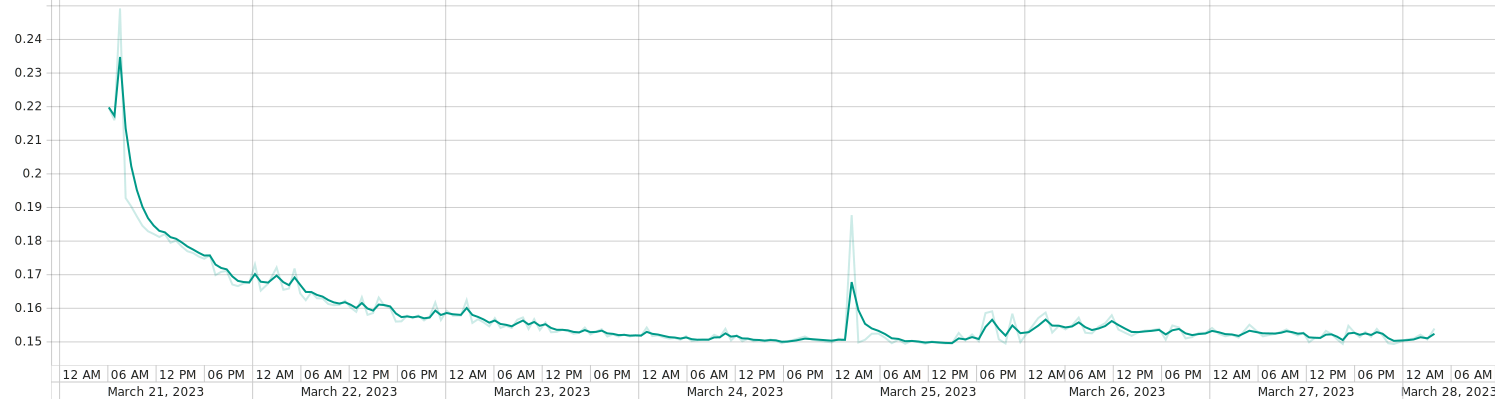
\includegraphics[width=0.75\textwidth]{images/val_loss.png}
     \caption{Graph showing validation dataset loss against the real-world time. Graph generated using Tensorboard from logs generated by PyTorch Lightning \citep{Falcon_PyTorch_Lightning_2019}}
     \label{fig:full_scan_tensorboard}
\end{figure}

\subsection{Results}

After training the model, averaged DSC and HD scores were computed on the validation set for each organ using the model from the last epoch. Computing the scores per organ allows for a higher-fidelity examination of the results to see what organs the model is failing on. This information could be used to further refine the model in future. Additionally, macro-averaged DSC and HD scores were computed to compare with the model computed in earlier evaluations. These results can be seen in Table \ref{tab:full_scan_test}.

Since this model is to be compared with literature, test dataset scores were also computed in the same way, using the data split off from the defined training set - described in Section \ref{sec:custom_dataloader}. Additionally, inferences were computed for each scan in the AMOS-defined test dataset so that they could be evaluated and listed on the AMOS leaderboard. The final place for the Perceiver IO model on the multi-modality AMOS leaderboard was third, and the computed average DSC for the AMOS test set was \num{0.0114}.

On top of these evaluations, the model’s average inference time for a single inference of batch size $1$ was found to be \num{2.3680281897385913} seconds. This was achieved on a single NVIDIA RTX 3080 GPU. A comparison of an example inference and the ground truth values is shown in Figure \ref{fig:full_scan_example_results}.

\begin{table}[]
\caption{Macro-averaged Dice coefficient and Hausdorff Distance metrics computed for each organ across all scans in the validation and test datasets for the full-scan Perceiver IO model using baseline parameters and multi-modality data} \label{tab:full_scan_test}
\begin{tabular}{lllll}
                             & \multicolumn{2}{c}{\textbf{Validation}}                                      & \multicolumn{2}{c}{\textbf{Test}}                                            \\
\textbf{}                    & \multicolumn{1}{c}{\textbf{Avg. DSC}} & \multicolumn{1}{c}{\textbf{Avg. HD}} & \multicolumn{1}{c}{\textbf{Avg. DSC}} & \multicolumn{1}{c}{\textbf{Avg. HD}} \\
\textbf{Spleen}              & \num{0.02273342347} & \num{12.65616588} & \num{0.002551293575} & \num{5.999422889} \\
\textbf{Right Kidney}        & \num{0.07862039172} & \num{33.9510022} & \num{0.04086970348} & \num{24.17037196} \\
\textbf{Left Kidney}         & \num{0.05877151864} & \num{35.13106784} & \num{0.02647333512} & \num{25.53405809} \\
\textbf{Gall Bladder}        & \num{0.0000000} & \num{27.06081621} & \num{0.0000000} & \num{6.59429694} \\
\textbf{Esophagus}           & \num{0.001508405073} & \num{5.777476939} & \num{0.0000000} & \num{0.0000000} \\
\textbf{Liver}               & \num{0.06771474167} & \num{30.46165037} & \num{0.01219563391} & \num{30.59217912} \\
\textbf{Stomach}             & \num{0.01014189373} & \num{18.65147704} & \num{0.00002443362849} & \num{3.61286487} \\
\textbf{Arota}               & \num{0.007851799587} & \num{24.01414692} & \num{0.003901916328} & \num{24.6967231} \\
\textbf{Postcava}            & \num{0.03608751075} & \num{37.48870022} & \num{0.01347900966} & \num{28.61223738} \\
\textbf{Pancreas}            & \num{0.01003005434} & \num{34.09721137} & \num{0.001730805429} & \num{23.03841023} \\
\textbf{Right Adrenal Gland} & \num{0.001294870046} & \num{7.35354882} & \num{0.0000000} & \num{0.8328162305} \\
\textbf{Left Adrenal Gland}  & \num{0.001812602194} & \num{11.24700121} & \num{0.0001868298913} & \num{8.785272272} \\
\textbf{Duodenum}            & \num{0.02653397724} & \num{46.84525031} & \num{0.004537575272} & \num{29.03490878} \\
\textbf{Bladder}             & \num{0.000001656095259} & \num{4.198336134} & \num{0.0000000} & \num{0.0000000} \\
\textbf{Prostate/Uterus}     & \num{0.008327858285} & \num{11.81909781} & \num{0.0000000} & \num{3.894359358}\\
\textbf{Macro}               & \num{0.02209538019} & \num{22.71686329} & \num{0.007063369087} & \num{14.35986141}
\end{tabular}
\end{table}

\begin{figure}[htb] 
    \centering

    \begin{subfigure}[b]{0.45\textwidth}
        \includegraphics[width=\textwidth]{images/liver_gt_1.png}
        \caption{Figure showing the axial ground-truth segmentations of the liver and surrounding area at slice $60$}
        \label{fig:full_scan_example_results_liver_gt_1}
    \end{subfigure}
    ~
    \begin{subfigure}[b]{0.45\textwidth}
        \includegraphics[width=\textwidth]{images/liver_inf_1.png}
        \caption{Figure showing the axial inference segmentations of the liver and surrounding area at slice $60$}
        \label{fig:full_scan_example_results_liver_inf_1}
    \end{subfigure} \\
    \begin{subfigure}[b]{0.45\textwidth}
        \includegraphics[width=\textwidth]{images/kidneys_gt.png}
        \caption{Figure showing the axial ground-truth segmentations of the liver and surrounding area at slice $45$}
        \label{fig:full_scan_example_results_kidney_gt}
    \end{subfigure}
    ~
    \begin{subfigure}[b]{0.45\textwidth}
        \includegraphics[width=\textwidth]{images/kidneys_inf.png}
        \caption{Figure showing the axial inference segmentations of the kidneys and surrounding area at slice $45$}
        \label{fig:full_scan_example_results_kidney_inf}
    \end{subfigure} \\

    \begin{subfigure}[b]{0.45\textwidth}
        \includegraphics[width=\textwidth]{images/liver_gt_2.png}
        \caption{Figure showing the coronal ground-truth segmentations of the liver and kidneys at slice $201$}
        \label{fig:full_scan_example_results_liver_gt_2}
    \end{subfigure}
    ~
    \begin{subfigure}[b]{0.45\textwidth}
        \includegraphics[width=\textwidth]{images/liver_inf_2.png}
        \caption{Figure showing the coronal inference segmentations of the liver and kidneys at slice $201$}
        \label{fig:full_scan_example_results_liver_inf_2}
    \end{subfigure}

    \caption{Scan 123 from the AMOS dataset \citep{ji2022amos}, visualised using ITK-SNAP \citep{itksnap}. Screenshots centred on the kidneys and livers across the axial and coronal planes to highlight the differences between the ground truth segmentations and the inference segmentations} \label{fig:full_scan_example_results}
\end{figure}

\section{Ablation Studies} \label{sec:ablation_studies}

To further investigate and evaluate the features added to make the Perceiver IO architecture more effective at medical image segmentation, ablation studies were performed on the inclusion of recursive and overlapping slices. The models trained used the same parameters as the baseline model, as training was faster and the results were comparable. We also trained the models for 350 epochs, allowing them to converge and inference optimally. The models were also trained on only 12 slices to allow for faster training while still having long-range relationships in the data. Additionally, the models with the highest DSC on the validation set were used for the inferences as opposed to the last model trained, which may have begun overfitting to the training set.

\subsection{Results}

The models trained and compared include the baseline model but with two recursive and two overlapping slices, zero recursive and two overlapping, two recursive and zero overlapping, and zero recursive or overlapping slices. This forms a Punnett square for these parameters, shown in Tables \ref{tab:ablation_results_dsc} and \ref{tab:ablation_results_hd} with macro-averaged Dice coefficient and Hausdorff distances on the validation set for each model, respectively.

\begin{table}[]
\caption{Macro-averaged Dice coefficients across all organ labels in the validation set for each model trained during the ablation study} \label{tab:ablation_results_dsc}
\begin{tabular}{lll}
\textbf{}                        & \textbf{Two Recursive Slices} & \textbf{Zero Recursive Slices} \\
\textbf{Two Overlapping Slices}  & \num{0.031792874}                              & \num{0.029911231}                               \\
\textbf{Zero Overlapping Slices} & \textbf{\num{0.040539090}}                              & \num{0.022941925}                              
\end{tabular}
\end{table}

\begin{table}[]
\caption{Macro-averaged Hausdorff Distances across all organ labels in the validation set for each model trained during the ablation study} \label{tab:ablation_results_hd}
\begin{tabular}{lll}
\textbf{}                        & \textbf{Two Recursive Slices} & \textbf{Zero Recursive Slices} \\
\textbf{Two Overlapping Slices}  & \num{28.758401609}                              & \num{38.302144268}                               \\
\textbf{Zero Overlapping Slices} & \num{26.29081229}                              & \textbf{\num{14.785593228}}                              
\end{tabular}
\end{table}

Further, the average inference times for each model were computed to see if any improvements in performance may be at the cost of time to inference. These times are shown in Table \ref{tab:ablation_results_inference}.

\begin{table}[]
\caption{Mean inference times in seconds across all scans in the validation set for each model trained during the ablation study; smaller is better} \label{tab:ablation_results_inference}
\begin{tabular}{lll}
\textbf{}                        & \textbf{Two Recursive Slices} & \textbf{Zero Recursive Slices} \\
\textbf{Two Overlapping Slices}  & \num{0.21218538999557496}                              & \num{0.21741403341293336}                               \\
\textbf{Zero Overlapping Slices} & \num{0.1504565715789795}                              & \textbf{\num{0.1414994168281555}}                              
\end{tabular}
\end{table}

\section{Additional Observations}

During the evaluation of the model, particularly anomalous results were identified multiple times. When there is no organ data in certain areas, such as a region of the body that does not contain any labelled organs, the network still infers that organs are present. This can be seen in Figure \ref{fig:full_scan_example_results_liver_inf_2} where the network attempts to infer that the spleen is present in the lungs. This could result from the network wrongly learning where to attend to and attending to areas other than the spleen for information about the spleen.

However, this style of mis-inferencing has also been found to be present in areas with no surrounding data. This can be seen in Figure \ref{fig:additional_mis_inference} where several labels are mis-inferenced, with large distances between them, showing that no information should be passed into the network through the inputs. However, namely with the Prostate/Uterus classification, the Perceiver IO’s classifications are approximately where the organ would have been located had they been included in the scan.

\begin{figure}[htb] 
    \centering

    \begin{subfigure}[b]{0.45\textwidth}
        \includegraphics[width=\textwidth]{images/ghost_1.png}
        \caption{Figure showing mis-inferenced segmentations of the Prostate/Uterus label (the larger) and the Bladder label on the axial plane}
        \label{fig:additional_mis_inference_ghost_1}
    \end{subfigure}
    ~
    \begin{subfigure}[b]{0.45\textwidth}
        \includegraphics[width=\textwidth]{images/ghost_12.png}
        \caption{Figure showing mis-inferenced segmentations of the Prostate/Uterus label on the coronal plane to show its relation to the scan data}
        \label{fig:additional_mis_inference_ghost_12}
    \end{subfigure}
    \\
    \begin{subfigure}[b]{0.45\textwidth}
        \includegraphics[width=\textwidth]{images/ghost_2.png}
        \caption{Figure showing a mis-inferenced segmentation of the Gall Bladder on the axial plane}
        \label{fig:additional_mis_inference_ghost_2}
    \end{subfigure}
    ~
    \begin{subfigure}[b]{0.45\textwidth}
        \includegraphics[width=\textwidth]{images/ghost_22.png}
        \caption{Figure showing a mis-inferenced segmentation of the Gall Bladder on the coronal plane to show its relation to the scan data}
        \label{fig:additional_mis_inference_ghost_22}
    \end{subfigure}

    \caption{Scan 573 from the AMOS dataset \citep{ji2022amos}, visualised using ITK-SNAP \citep{itksnap} showing mis-inferences of the Prostate/Uterus, Bladder, and Gall Bladder in the presence of no data.} \label{fig:additional_mis_inference}
\end{figure}

\section{Discussion}

\subsection{Parameter Optimisation}

It can be seen from Table \ref{tab:parameter_optimisation_results} that the parameter optimisation has improved Perceiver IO’s results in the Dice coefficient metric and decreased its loss. This shows that the method for optimising the parameters was applied effectively. However, the optimised model does not perform better in the Hausdorff distance metric, showing that although there was a small increase in the DSC scores, the optimised model is not significantly better than the baseline model. Additionally, due to the increase in the number of parameters and, by extension, the inference time, the optimised model is not worth using for medical image segmentation over the baseline model.

Although the parameter optimisation did not lead to further refinement in this paper, this paper proves that this technique can be used to optimise the parameters of the Perceiver IO network. Allowing the parameter optimisation to run longer would further improve the results and, as discussed in Section \ref{sec:future_work}, could lead to substantial improvements in the network’s performance.

\subsection{Multi-Modality}

The results of the multi-modality evaluation show that the model trained with multiple data sources not only performs as well as the one trained with only one, but performs significantly better. This is shown by the clear improvements in the DSC and HD metrics, with a \num{181.2373504487749}\% increase and a \num{49.95416357146475}\% decrease, respectively. As such, we can say that the Perceiver IO network performs significantly better when exposed to multi-modality data than single-modality.

This could be because the multi-modality model had far more scans to train on - 168 instead of only 140 - which would allow the network to improve the quality of its training; in turn, improving its inference and generalisation capabilities. As such, the improvements in the results are likely due to more training data being available. However, the improvement is still beneficial as it shows that the Perceiver IO model can effectively utilise MRI and CT scan data to perform meaningful inferences on both. This shows that the Perceiver IO network can effectively generalise to multi-modality data through its expressive latent array. In turn, this could allow trained models to effectively infer either CT or MRI data interchangeably. As stated by the AMOS challenge \citep{ji2022amos}, this could help spur deployment and real-world usage of such a segmentation solution. 

Furthermore, since the Perceiver IO network can effectively train using both modalities, future training jobs for Perceiver-based networks can also be done using multi-modality data. This will allow these networks to have far more data to train using, helping to improve their performances further. This is especially useful for the medical image segmentation field due to the relative scarcity and difficulty in collecting data to train models. As such, Peceiver-based networks that train on multiple data-source may easily outperform non-generalisable, single-modality networks  due to their ability to effectively train using more data.

\subsection{Full-Scan Inferences and Additional Observations}

From the full-scan evaluation results, we found that the Perceiver IO network is able to create meaningful, multi-label, multi-modality segmentations. However, compared to state-of-the-art networks, its performance is lacking, coming third/last on the AMOS multi-modality leaderboard and failing to compute any accurate inferences on several organs, namely the gall bladder and bladder.

This could be due to several reasons. However, the most likely is because the Perceiver IO architecture usage described in this paper is far more simplistic than the current state-of-the-art biomedical segmentation networks. This concurs with the original Perceiver paper's findings: It performs better than generic solutions but rarely better than the state-of-the-art custom solutions \citep{perceiver}. As such, the Perceiver architecture is not directly producing competitive biomedical segmentations in its current state.

However, as shown in Figure \ref{fig:additional_mis_inference_ghost_22}, it is learning how to predict organs based on very little input information - sometimes without any. As such, we still believe that it is learning an expressive array that is, by its default nature, modelling the human body based on spatial information. As such, the Perceiver network can be seen to tackle the lack of long-range spatial and morphological dependencies seen with other network architectures. From this, we believe that the Perceiver IO architecture does warrant further investigation into its capabilities, further described in Section \ref{sec:future_work}. 

\subsection{Ablation Studies}

The ablation studies performed on the network show that the current implementation of recursive slices significantly improves the Perceiver IO architecture's performance - increasing the DSC metric by up to \num{176.7030883415407}\%. Recursive slices also decreased the HD metric by \num{24.91699313809289}\% when used with two overlapping slices. There also does not appear to be any significant increase in inference times when using recursive slices, making their inclusion in the network only a benefit and confirming that they are effective in improving the network's performance. This finding agrees with similar research on recursive inferences using the U-Net architecture.

Unlike their recursive counterparts, overlapping slices appear to decrease network performance when viewing the DSC metric. This is particularly interesting as they were initially employed to increase the performance of the Perceiver IO model. Overlapping slices were implemented to help to smooth the edges of the inferred labels, as they were seen to be very rough in earlier implementations of the architecture. As shown in the results, despite the decrease in the DSC, there is also a decrease in the Hausdorff distance in all cases. This indicates that the inclusion of overlapping slices does successfully improve the edges of the segmentations. This is at the cost of the segmentations' overall accuracy. Additionally, overlapping slices do significantly increase the inference times of the models, likely due to the increased number of forward passes that must be completed to infer the same number of scan slices. As such, overlapping slices should not be utilised in future research on this task with the Perceiver architecture. This is with the exception of cases where the network performs poorly at label edges, which may occur with more complex and accurate models. Additionally, we believe it should be noted that this implementation of overlapping scans is one of many forms that overlapping could take. We briefly discuss one such alternative approach that could be explored in future research in Section \ref{sec:future_work}.

%==================================================================================================================================
\chapter{Conclusion} \label{chap:conclusion}

% Summarise the whole project for a lazy reader who didn't read the rest (e.g. a prize-awarding committee). This chapter should be short in most dissertations; maybe one to three pages.
% \section{Guidance}
% \begin{itemize}
%     \item
%         Summarise briefly and fairly.
%     \item
%         You should be addressing the general problem you introduced in the
%         Introduction.        
%     \item
%         Include summary of concrete results (``the new compiler ran 2x
%         faster'')
% \end{itemize}

% Summarise the whole project for a lazy reader who didn't read the rest (e.g. a prize-awarding committee). This chapter should be short in most dissertations; maybe one to three pages.
% \section{Guidance}
% \begin{itemize}
%     \item
%         Summarise briefly and fairly.
%     \item
%         You should be addressing the general problem you introduced in the
%         Introduction.        
%     \item
%         Include summary of concrete results (``the new compiler ran 2x
%         faster'')
% \end{itemize}

\section{Summary}
% Summarise what you did; answer the general questions you asked in the introduction. What did you achieve? Briefly describe what was built and summarise the evaluation results.

In this paper, a model based on the Perceiver IO architecture has been built to create medical image segmentations for multi-label abdominal CT and MRI scans. This model’s parameters have then been shown to be optimisable using a derivative-free optimisation algorithm, shown by a decrease in loss of \num{48.72986708138669}\%. The Perceiver IO model has also been shown to generalise to multiple modalities effectively, producing results \num{181.2373504487749}\% better when trained on multiple modalities instead of a single modality when compared with a standard metric; the macro-averaged Dice coefficient. Additionally, two extensions to the Perceiver IO architecture - recursive and overlapping slices - have been found to improve the network's performance by up to \num{176.7030883415407}\% when compared with the same metric.

When comparing the Perceiver IO architecture’s results to state-of-the-art models, however, we see that the model does not perform to the same standard despite the parameter optimisation, additional features, and multi-modality training: Our trained model came third/last in a standardised online leaderboard for the abdominal segmentation dataset used for the comparative evaluations with a macro-averaged Dice coefficient of \num{0.0114}. As such, in this current state, we do not believe that the Perceiver IO can be used to create competitive biomedical image segmentations.

Despite these undesirable results compared to the current literature, we believe this paper is an effective exploratory work highlighting that the Perceiver architecture should be explored further. Our results show that this architecture is receptive to novel extensions and is incredibly effective when generalising to multi-modality data. As such, we believe that with further refinements to the network architecture and inspiration from existing state-of-the-art systems, such as U-Net, the Perceiver IO architecture could outperform current architectures. From this, we foresee this paper bringing about many opportunities for future research based on these initial evaluations.

% \section{Reflection}
% Discuss what went well and what didn't and how you would do things differently if you did this project again.

\section{Future Work} \label{sec:future_work}
% Discuss what you would do if you could take this further -- where would the interesting directions to go next be? (e.g. you got another year to work on it, or you started a company to work on this, or you pursued a PhD on this topic)

These conclusions show that the Perceiver IO network could have a place in biomedical image segmentation tasks. As such, better exploration of its applications is necessary to guarantee that the field continues to grow and innovate. This chapter proposes several ideas for how the Perceiver IO network can be further investigated.

The primary recommendation is to continue the work outlined in this paper, allowing for more resources and time to train the models. This would come in the form of increasing the budget for optimising the network’s parameters and training the final full-scan segmentation model until validation loss increases. Additionally, if more computational resources could be utilised to train the model, a deeper and more expressive model should be trained and evaluated. A model such as this may have better segmentation abilities than the models trained in this paper, further solidifying the need to investigate the Perceiver architecture further.

One recommendation for further research builds on what has already been achieved by vision transformers. Firstly, we would recommend research be completed to evaluate if the Perceiver architecture would work effectively as part of a hierarchical sliding-window transformer, like the Swin transformers developed by \cite{liu2021swin}. From this development, it would be useful to evaluate if these new integrations of the Perceiver architecture can produce higher-quality segmentations than a direct application of the architecture, shown in this paper.

Further, with the success of the U-Net architecture, integrating the Perceiver transformers could yield improved results. As seen when integrating vision transformers with the Swin-UNet architecture, impressive results were gained \citep{cao2023swin}. Therefore, integrating the Perceiver IO network into U-Net would hopefully improve results significantly as well. Additionally, due to the Perceiver IO architecture’s separated encoder and decoder, there would be no need for the patch merging and embeddings used in the original Swin-UNet. This could allow for the latent expression of the network to be utilised to the fullest extent, possibly yielding far improved and generalisable results.

Once a U-Net style model has been created, further research can be completed to investigate how several existing improvements to the U-Net model affect the Perceiver U-Net model. Touched on this paper, an example could be including recursive information between slabs. In this paper, recursion was implemented as the output of the full network stacked on top of the next set of inputs; however, this definition could be extended to include recursion between each Perceiver model in the encoder and decoder levels. This could further improve the attention and performance of the model across slabs as more of the expressive latent representations can be persisted \citep{wang2019recurrent}. On top of recursion, other techniques, such as overlapping voxels from independent sagittal, coronal, and axial segmentations could improve the outputted segmentations, although at the expense of having to train three times as many models for each plane.

Additionally, a better loss function could improve the quality of the model’s segmentations. Borrowing from image and video generation research, a model could be trained in parallel with the segmentation-generating model to determine the authenticity of a segmentation. This second model could be used adversarially to reject low-quality image segmentations, raising the bar for the quality of the segmentations the model must generate. In turn, this should improve the quality of the segmentations created by biomedical segmentation models, although at the cost of even greater computational requirements.

On top of the replication and further research to be completed, several other advances can help to improve biomedical segmentation based on this research. Better preprocessing pipelines could be defined to help improve the training of models due to the lack of biomedical data to train on. Techniques such as random noise, blurring, and random cropping could create multiple possible images to train with from one - allowing for better training. Several Perceiver IO models should be pretrained to allow for more rapid development and testing of their integrations. Additional techniques to improve the Perceiver model’s efficiency and effectiveness should also be integrated, such as checkpointing, to allow deeper models to be trained on hardware with less memory. Further, batching could also help stabilise and speed up model training, but may only be possible on systems with large amounts of VRAM.

%==================================================================================================================================
%
% 
%==================================================================================================================================
%  APPENDICES  

\begin{appendices}

\chapter{User Manual} \label{chap:appendices}

Below is the information on how to run the Perceiver IO data processing, training, and inferencing, which is also included as a markdown file with the source code:

\section{Development}

\subsection{Prerequisites}

\begin{itemize}
  \item{Miniconda installed}
  \item{Running on Ubuntu 22.04 (development was completed on WSL but should not be necessary for running)}
  \item{amos22 dataset: \url{https://zenodo.org/record/7155725#.Y_7WqHbP1D-} stored somewhere. where the path is important, it will be noted.}
\end{itemize}

\subsection{Creating environment}

This is required for all further steps, which all assume that the conda \lstinline{perceiver-io} environment is activated already

\begin{lstlisting}[language=bash]
cd perceiver-io
conda env create -f environment.yml
conda activate perceiver-io
python -m pip install poetry -U
poetry install --all-extras
poetry build
\end{lstlisting}

\subsection{Preprocessing dataset}

This will run automatically when the dataset is loaded, but can be ran individually as well. It assumes that the dataset can be found at \lstinline{/mnt/d/amos22}, this must be changed inside of \lstinline{perceiver/scripts/segmentation/preproc.py} if not true:

\begin{lstlisting}[language=bash]
cd perceiver-io
sh scripts/miccai/preproc.sh
\end{lstlisting}

\subsection{Running training}

\begin{lstlisting}[language=bash]
cd perceiver-io
cp -r /path/to/amos22 /dev/shm # load amos22 dataset into shared memory. not all data must be loaded to memory, only, imagesTr_preprocessed/* labelsTr_preprocessed/*, dataset.json, and several empty folders: [imagesTr, imagesVa, imagesVa_preprocessed, labelsTr, labelsVa, labelsVa_preprocessed]
sh scripts/miccai/train.sh
\end{lstlisting}

\subsection{Running inference}

\begin{lstlisting}[language=bash]
cd perceiver-io
cp -r /path/to/amos22 /dev/shm # load amos22 dataset into shared memory. not all data must be loaded to memory, only, imagesTr_preprocessed/* labelsTr_preprocessed/*, dataset.json, and several empty folders: [imagesTr, imagesVa, imagesVa_preprocessed, labelsTr, labelsVa, labelsVa_preprocessed] This obviously depends on what dataset split is to be inferenced
python -m perceiver.scripts.segmentation.inference # several configuration parameters can be changed in the GLOBALS at the start of the corresponding file
\end{lstlisting}

\subsection{Running automated parameter optimisation}

\begin{lstlisting}[language=bash]
cd perceiver-io
cp -r /path/to/amos22 /dev/shm # load amos22 dataset into shared memory. not all data must be loaded to memory, only, imagesTr_preprocessed/* labelsTr_preprocessed/*, dataset.json, and several empty folders: [imagesTr, imagesVa, imagesVa_preprocessed, labelsTr, labelsVa, labelsVa_preprocessed]
sh scripts/miccai/automated_optimise.sh 2>&1 | tee log.txt # optimal parameters will be printed to the console, hence recommending using the use of tee
\end{lstlisting}

\section{Docker deployment}

\subsection{Prerequisite}

\begin{itemize}
  \item{docker installed}
  \item{trained model weights}
  \item{image used for coregistration (normally found in \\ \lstinline{amos22/imagesTr_preprocessed/coregistration_image.nii.gz})}
\end{itemize}

\subsection{Building image}

\begin{lstlisting}[language=bash]
cd perceiver-io
sh scripts/docker_build.sh path/to/model.ckpt path/to/coregistration_image.nii.gz tagname
\end{lstlisting}

\subsection{Deploying/pushing iamge}

\begin{lstlisting}[language=bash]
docker push tagname
\end{lstlisting}

\subsection{Using docker image for inference}

There is already a prebuilt docker image deployed on ghcr.io. It can be pulled using:

\begin{lstlisting}[language=bash]
docker pull ghcr.io/questiowo/miccai-perceiver-io
\end{lstlisting}

This may require logging in, information on how to do so can be found in GitHub documentation: \url{https://docs.github.com/en/packages/working-with-a-github-packages-registry/working-with-the-container-registry#authenticating-with-a-personal-access-token-classic}

Information on how to correctly run the docker image using GPU acceleration can be found in the AMOS22 docker submission guidelines here \url{https://github.com/JiYuanFeng/AMOS/tree/docker#step-4-run-a-container-from-a-created-docker-image}.

\subsection{Using OpenShift Compute Cluster}

The OpenShift compute cluster GPUs can be used to train on by using the associated \lstinline{Dockerfile.XXX} docker image. These are currently uploaded, ready for use on hub.docker.com: \url{https://hub.docker.com/search?q=perceiver-io}.

The configuration yaml files are included in the project as \lstinline{job-perceiver-io-*.yaml}. The jobs expect the \lstinline{amos22} dataset to be uploaded to an associated NFS store, which can be attached at \lstinline{/volume/}. This is configured in the yaml-file and can be adjusted to new users easily.

The docker commands are written into each Dockerfile and are not observant to different numbers of GPGPUs. This means that if a cluster with (not 2) GPUs is available, the docker image has to be rebuilt, repushed, and the job restarted with the correct batch size and devices. Alternatively, the yaml configuration files can be extended to instead have the training job script inside the configuration file instead of the Dockerfile, however, an example is not included of that.

\end{appendices}

%==================================================================================================================================
%   BIBLIOGRAPHY   

% The bibliography style is agsm (Harvard)
% The bibliography always appears last, after the appendices.

\bibliographystyle{agsm}

% Force the bibliography not to be numbered
\renewcommand{\thechapter}{0} 
\bibliography{l4proj}

\end{document}
